\documentclass{anstrans}
%%%%%%%%%%%%%%%%%%%%%%%%%%%%%%%%%%%
\title{Demonstration of Demand Driven Deployment Capabilities in \Cyclus}
\author{Gwendolyn J. Chee$^1$, Jin Whan Bae$^2$, Robert R. Flanagan$^3$, Roberto E. Fairhurst Agosta$^1$ and Kathryn D. Huff$^1$}

\institute{
$^1$Dept. of Nuclear, Plasma and Radiological Engineering, University of Illinois at Urbana-Champaign \\
$^2$ Oak Ridge National Laboratory, Oak Ridge, TN, United States \\
$^3$Nuclear Engineering Program, University of South Carolina \\

gchee2@illinois.edu
}

%%%% packages and definitions (optional)
\usepackage[utf8]{inputenc}
\usepackage{graphicx} % allows inclusion of graphics
\usepackage{booktabs} % nice rules (thick lines) for tables
\usepackage{microtype} % improves typography for PDF
\usepackage{xspace}
\usepackage{tabularx}
\usepackage{subcaption}
\usepackage{enumitem}
\usepackage{placeins}
\usepackage{multirow}
\usepackage{amsmath}
\usepackage[acronym,toc]{glossaries}
%\newacronym{<++>}{<++>}{<++>}
\newacronym[longplural={metric tons of heavy metal}]{MTHM}{MTHM}{metric ton of heavy metal}
\newacronym{ABM}{ABM}{agent-based modeling}
\newacronym{ACDIS}{ACDIS}{Program in Arms Control \& Domestic and International Security}
\newacronym{AHTR}{AHTR}{Advanced High Temperature Reactor}
\newacronym{ANDRA}{ANDRA}{Agence Nationale pour la gestion des D\'echets RAdioactifs, the French National Agency for Radioactive Waste Management}
\newacronym{ANL}{ANL}{Argonne National Laboratory}
\newacronym{API}{API}{application programming interface}
\newacronym{ARE}{ARE}{Aircraft Reactor Experiment}
\newacronym{ARFC}{ARFC}{Advanced Reactors and Fuel Cycles}
\newacronym{ASME}{ASME}{American Society of Mechanical Engineers}
\newacronym{ATWS}{ATWS}{Anticipated Transient Without Scram}
\newacronym{BDBE}{BDBE}{Beyond Design Basis Event}
\newacronym{BIDS}{BIDS}{Berkeley Institute for Data Science}
\newacronym{CAFCA}{CAFCA}{ Code for Advanced Fuel Cycles Assessment }
\newacronym{CDTN}{CDTN}{Centro de Desenvolvimento da Tecnologia Nuclear}
\newacronym{CEA}{CEA}{Commissariat \`a l'\'Energie Atomique et aux \'Energies Alternatives}
\newacronym{CI}{CI}{continuous integration}
\newacronym{CNEN}{CNEN}{Comiss\~{a}o Nacional de Energia Nuclear}
\newacronym{CNERG}{CNERG}{Computational Nuclear Engineering Research Group}
\newacronym{COSI}{COSI}{Commelini-Sicard}
\newacronym{COTS}{COTS}{commercial, off-the-shelf}
\newacronym{CSNF}{CSNF}{commercial spent nuclear fuel}
\newacronym{CTAH}{CTAHs}{Coiled Tube Air Heaters}
\newacronym{CUBIT}{CUBIT}{CUBIT Geometry and Mesh Generation Toolkit}
\newacronym{CURIE}{CURIE}{Centralized Used Fuel Resource for Information Exchange}
\newacronym{DAG}{DAG}{directed acyclic graph}
\newacronym{DANESS}{DANESS}{Dynamic Analysis of Nuclear Energy System Strategies}
\newacronym{DBE}{DBE}{Design Basis Event}
\newacronym{DESAE}{DESAE}{Dynamic Analysis of Nuclear Energy Systems Strategies}
\newacronym{DHS}{DHS}{Department of Homeland Security}
\newacronym{DOE}{DOE}{Department of Energy}
\newacronym{DRACS}{DRACS}{Direct Reactor Auxiliary Cooling System}
\newacronym{DRE}{DRE}{dynamic resource exchange}
\newacronym{DSNF}{DSNF}{DOE spent nuclear fuel}
\newacronym{DYMOND}{DYMOND}{Dynamic Model of Nuclear Development }
\newacronym{EBS}{EBS}{Engineered Barrier System}
\newacronym{EDZ}{EDZ}{Excavation Disturbed Zone}
\newacronym{EIA}{EIA}{U.S. Energy Information Administration}
\newacronym{EPA}{EPA}{Environmental Protection Agency}
\newacronym{EP}{EP}{Engineering Physics}
\newacronym{FCO}{FCO}{Fuel Cycle Options}
\newacronym{FCT}{FCT}{Fuel Cycle Technology}
\newacronym{FEHM}{FEHM}{Finite Element Heat and Mass Transfer}
\newacronym{FEPs}{FEPs}{Features, Events, and Processes}
\newacronym{FHR}{FHR}{Fluoride-Salt-Cooled High-Temperature Reactor}
\newacronym{FLiBe}{FLiBe}{Fluoride-Lithium-Beryllium}
\newacronym{GDSE}{GDSE}{Generic Disposal System Environment}
\newacronym{GDSM}{GDSM}{Generic Disposal System Model}
\newacronym{GENIUSv1}{GENIUSv1}{Global Evaluation of Nuclear Infrastructure Utilization Scenarios, Version 1}
\newacronym{GENIUSv2}{GENIUSv2}{Global Evaluation of Nuclear Infrastructure Utilization Scenarios, Version 2}
\newacronym{GENIUS}{GENIUS}{Global Evaluation of Nuclear Infrastructure Utilization Scenarios}
\newacronym{GPAM}{GPAM}{Generic Performance Assessment Model}
\newacronym{GRSAC}{GRSAC}{Graphite Reactor Severe Accident Code}
\newacronym{GUI}{GUI}{graphical user interface}
\newacronym{HLW}{HLW}{high level waste}
\newacronym{HPC}{HPC}{high-performance computing}
\newacronym{HTC}{HTC}{high-throughput computing}
\newacronym{HTGR}{HTGR}{High Temperature Gas-Cooled Reactor}
\newacronym{IAEA}{IAEA}{International Atomic Energy Agency}
\newacronym{IEMA}{IEMA}{Illinois Emergency Mangament Agency}
\newacronym{INL}{INL}{Idaho National Laboratory}
\newacronym{IPRR1}{IRP-R1}{Instituto de Pesquisas Radioativas Reator 1}
\newacronym{IRP}{IRP}{Integrated Research Project}
\newacronym{ISFSI}{ISFSI}{Independent Spent Fuel Storage Installation}
\newacronym{ISRG}{ISRG}{Independent Student Research Group}
\newacronym{JFNK}{JFNK}{Jacobian-Free Newton Krylov}
\newacronym{LANL}{LANL}{Los Alamos National Laboratory}
\newacronym{LBNL}{LBNL}{Lawrence Berkeley National Laboratory}
\newacronym{LCOE}{LCOE}{levelized cost of electricity}
\newacronym{LDRD}{LDRD}{laboratory directed research and development}
\newacronym{LFR}{LFR}{Lead-Cooled Fast Reactor}
\newacronym{LLNL}{LLNL}{Lawrence Livermore National Laboratory}
\newacronym{LMFBR}{LMFBR}{Liquid Metal Fast Breeder Reactor}
\newacronym{LOFC}{LOFC}{Loss of Forced Cooling}
\newacronym{LOHS}{LOHS}{Loss of Heat Sink}
\newacronym{LOLA}{LOLA}{Loss of Large Area}
\newacronym{LP}{LP}{linear program}
\newacronym{LWR}{LWR}{Light Water Reactor}
\newacronym{MA}{MA}{minor actinide}
\newacronym{MCNP}{MCNP}{Monte Carlo N-Particle code}
\newacronym{MILP}{MILP}{mixed-integer linear program}
\newacronym{MIT}{MIT}{the Massachusetts Institute of Technology}
\newacronym{MOAB}{MOAB}{Mesh-Oriented datABase}
\newacronym{MOOSE}{MOOSE}{Multiphysics Object-Oriented Simulation Environment}
\newacronym{MOX}{MOX}{mixed oxide}
\newacronym{MSBR}{MSBR}{Molten Salt Breeder Reactor}
\newacronym{MSRE}{MSRE}{Molten Salt Reactor Experiment}
\newacronym{MSR}{MSR}{Molten Salt Reactor}
\newacronym{NAGRA}{NAGRA}{National Cooperative for the Disposal of Radioactive Waste}
\newacronym{NEAMS}{NEAMS}{Nuclear Engineering Advanced Modeling and Simulation}
\newacronym{NEUP}{NEUP}{Nuclear Energy University Programs}
\newacronym{NFCSim}{NFCSim}{Nuclear Fuel Cycle Simulator}
\newacronym{NGNP}{NGNP}{Next Generation Nuclear Plant}
\newacronym{NMWPC}{NMWPC}{Nuclear MW Per Capita}
\newacronym{NNSA}{NNSA}{National Nuclear Security Administration}
\newacronym{NPRE}{NPRE}{Department of Nuclear, Plasma, and Radiological Engineering}
\newacronym{NQA1}{NQA-1}{Nuclear Quality Assurance - 1}
\newacronym{NRC}{NRC}{Nuclear Regulatory Commission}
\newacronym{NSF}{NSF}{National Science Foundation}
\newacronym{NSSC}{NSSC}{Nuclear Science and Security Consortium}
\newacronym{NUWASTE}{NUWASTE}{Nuclear Waste Assessment System for Technical Evaluation}
\newacronym{NWF}{NWF}{Nuclear Waste Fund}
\newacronym{NWTRB}{NWTRB}{Nuclear Waste Technical Review Board}
\newacronym{OCRWM}{OCRWM}{Office of Civilian Radioactive Waste Management}
\newacronym{ORION}{ORION}{ORION}
\newacronym{ORNL}{ORNL}{Oak Ridge National Laboratory}
\newacronym{PARCS}{PARCS}{Purdue Advanced Reactor Core Simulator}
\newacronym{PBAHTR}{PB-AHTR}{Pebble Bed Advanced High Temperature Reactor}
\newacronym{PBFHR}{PB-FHR}{Pebble-Bed Fluoride-Salt-Cooled High-Temperature Reactor}
\newacronym{PEI}{PEI}{Peak Environmental Impact}
\newacronym{PH}{PRONGHORN}{PRONGHORN}
\newacronym{PRKE}{PRKE}{Point Reactor Kinetics Equations}
\newacronym{PSPG}{PSPG}{Pressure-Stabilizing/Petrov-Galerkin}
\newacronym{PWAR}{PWAR}{Pratt and Whitney Aircraft Reactor}
\newacronym{PWR}{PWR}{Pressurized Water Reactor}
\newacronym{PyNE}{PyNE}{Python toolkit for Nuclear Engineering}
\newacronym{PyRK}{PyRK}{Python for Reactor Kinetics}
\newacronym{QA}{QA}{quality assurance}
\newacronym{RDD}{RD\&D}{Research Development and Demonstration}
\newacronym{RD}{R\&D}{Research and Development}
\newacronym{RELAP}{RELAP}{Reactor Excursion and Leak Analysis Program}
\newacronym{RIA}{RIA}{Reactivity Insertion Accident}
\newacronym{RIF}{RIF}{Region-Institution-Facility}
\newacronym{SFR}{SFR}{Sodium-Cooled Fast Reactor}
\newacronym{SINDAG}{SINDA{\textbackslash}G}{Systems Improved Numerical Differencing Analyzer $\backslash$ Gaski}
\newacronym{SKB}{SKB}{Svensk K\"{a}rnbr\"{a}nslehantering AB}
\newacronym{SNF}{SNF}{spent nuclear fuel}
\newacronym{SNL}{SNL}{Sandia National Laboratory}
\newacronym{STC}{STC}{specific temperature change}
\newacronym{SUPG}{SUPG}{Streamline-Upwind/Petrov-Galerkin}
\newacronym{SWF}{SWF}{Separations and Waste Forms}
\newacronym{SWU}{SWU}{Separative Work Unit}
\newacronym{TRIGA}{TRIGA}{Training Research Isotope General Atomic}
\newacronym{TRISO}{TRISO}{Tristructural Isotropic}
\newacronym{TSM}{TSM}{Total System Model}
\newacronym{TSPA}{TSPA}{Total System Performance Assessment for the Yucca Mountain License Application}
\newacronym{ThOX}{ThOX}{thorium oxide}
\newacronym{UFD}{UFD}{Used Fuel Disposition}
\newacronym{UML}{UML}{Unified Modeling Language}
\newacronym{UOX}{UOX}{uranium oxide}
\newacronym{UQ}{UQ}{uncertainty quantification}
\newacronym{US}{US}{United States}
\newacronym{UW}{UW}{University of Wisconsin}
\newacronym{VISION}{VISION}{the Verifiable Fuel Cycle Simulation Model}
\newacronym{VV}{V\&V}{verification and validation}
\newacronym{WIPP}{WIPP}{Waste Isolation Pilot Plant}
\newacronym{YMR}{YMR}{Yucca Mountain Repository Site}

\makeglossaries
\newcommand{\SN}{S$_N$}
\renewcommand{\vec}[1]{\bm{#1}} %vector is bold italic
\newcommand{\vd}{\bm{\cdot}} % slightly bold vector dot
\newcommand{\grad}{\vec{\nabla}} % gradient
\newcommand{\ud}{\mathop{}\!\mathrm{d}} % upright derivative symbol
\newcommand{\Cyclus}{\textsc{Cyclus}\xspace}%
\newcommand{\Cycamore}{\textsc{Cycamore}\xspace}%
\newcommand{\deploy}{\texttt{d3ploy}\xspace}%
\newcommand{\Deploy}{\texttt{D3ploy}\xspace}%
\newcolumntype{c}{>{\hsize=.56\hsize}X}
\newcolumntype{b}{>{\hsize=.7\hsize}X}
\newcolumntype{s}{>{\hsize=.74\hsize}X}
\newcolumntype{f}{>{\hsize=.1\hsize}X}
\newcolumntype{a}{>{\hsize=.45\hsize}X}
\usepackage{titlesec}
\titleformat*{\subsection}{\normalfont}
\usepackage{tikz}
\definecolor{illiniblue}{HTML}{437db6}
\definecolor{illiniorange}{HTML}{E38749}
\usetikzlibrary{shapes.geometric, arrows}
\tikzstyle{oblock} = [rectangle, draw, fill=illiniorange, 
text width=12em, text centered, rounded corners, minimum height=4em]
\tikzstyle{bblock} = [rectangle, draw, fill=illiniblue, 
text width=12em, text centered, rounded corners, minimum height=4em]
\tikzstyle{arrow} = [thick,->,>=stealth]

\begin{document}
%%%%%%%%%%%%%%%%%%%%%%%%%%%%%%%%%%%%%%%%%%%%%%%%%%%%%%%%%%%%%%%%%%%%
\section{Introduction}
For many fuel cycle simulators, it is currently up to the user 
to define a deployment scheme of supporting facilities to ensure 
that there is no gap in the supply chain. 
To ease setting up nuclear fuel cycle simulations, \gls{NFC}
simulators should bring demand responsive deployment decisions into 
the dynamics of the simulation logic \cite{huff_current_2017}. 
Thus, a next generation \gls{NFC} simulator should predictively and 
automatically deploy fuel cycle facilities to meet a user defined 
power demand. 

\Cyclus is an agent-based nuclear fuel cycle simulation framework 
\cite{huff_fundamental_2016}. 
In \Cyclus, each entity (i.e. Region, Institution, or Facility) in the 
fuel cycle is an agent. 
Region agents represent geographical or political areas that institution
and facility agents can be grouped into. 
Institution agents control the 
deployment and decommission of facility agents 
and represents legal operating organizations such as a 
utility, government, etc. \cite{huff_fundamental_2016}. 
Facility agents represent nuclear fuel cycle facilities. 
\Cycamore \cite{carlsen_cycamore_2014}
provides agents to represent process physics of various 
components in the nuclear fuel cycle (e.g. mine, fuel enrichment 
facility, reactor). 

The Demand-Driven \Cycamore Archetypes project 

\noindent
(NEUP-FY16-10512) 
aims to develop \Cyclus' demand-driven deployment capabilities. 
This capability is added as a \Cyclus Institution
agent that deploys facilities to meet the front-end and back-end 
fuel cycle demands based on a user-defined commodity demand. 
This demand-driven deployment capability is called 
\deploy. 

In this paper, we explain the capabilities of \deploy and
demonstrate how \deploy minimizes undersupply of all 
commodities in a few simulations while meeting key simulation 
constraints. 
Constant, linearly increasing, and sinusoidal power demand
transition scenarios are demonstrated. 
Insights are discussed to inform parameter 
input decisions for future work in setting up 
larger transition scenarios that include many facilities. 

%%%%%%%%%%%%%%%%%%%%%%%%%%%%%%%%%%%%%%%%%%%%%%%%%%%%%%%%%%%%%%%%%%%%
\section{D3ploy capabilities}
At each time step, \deploy predicts demand and supply of each 
commodity for the next time step.
Then, \deploy deploys facilities to meet predicted demand. 
\Deploy's primary objective is minimizing the number of time 
steps of undersupply of any commodity. 
Figure \ref{fig:flow} shows the flow of \deploy's logic at every time step. 

\begin{figure*}[!htb]
	\centering
	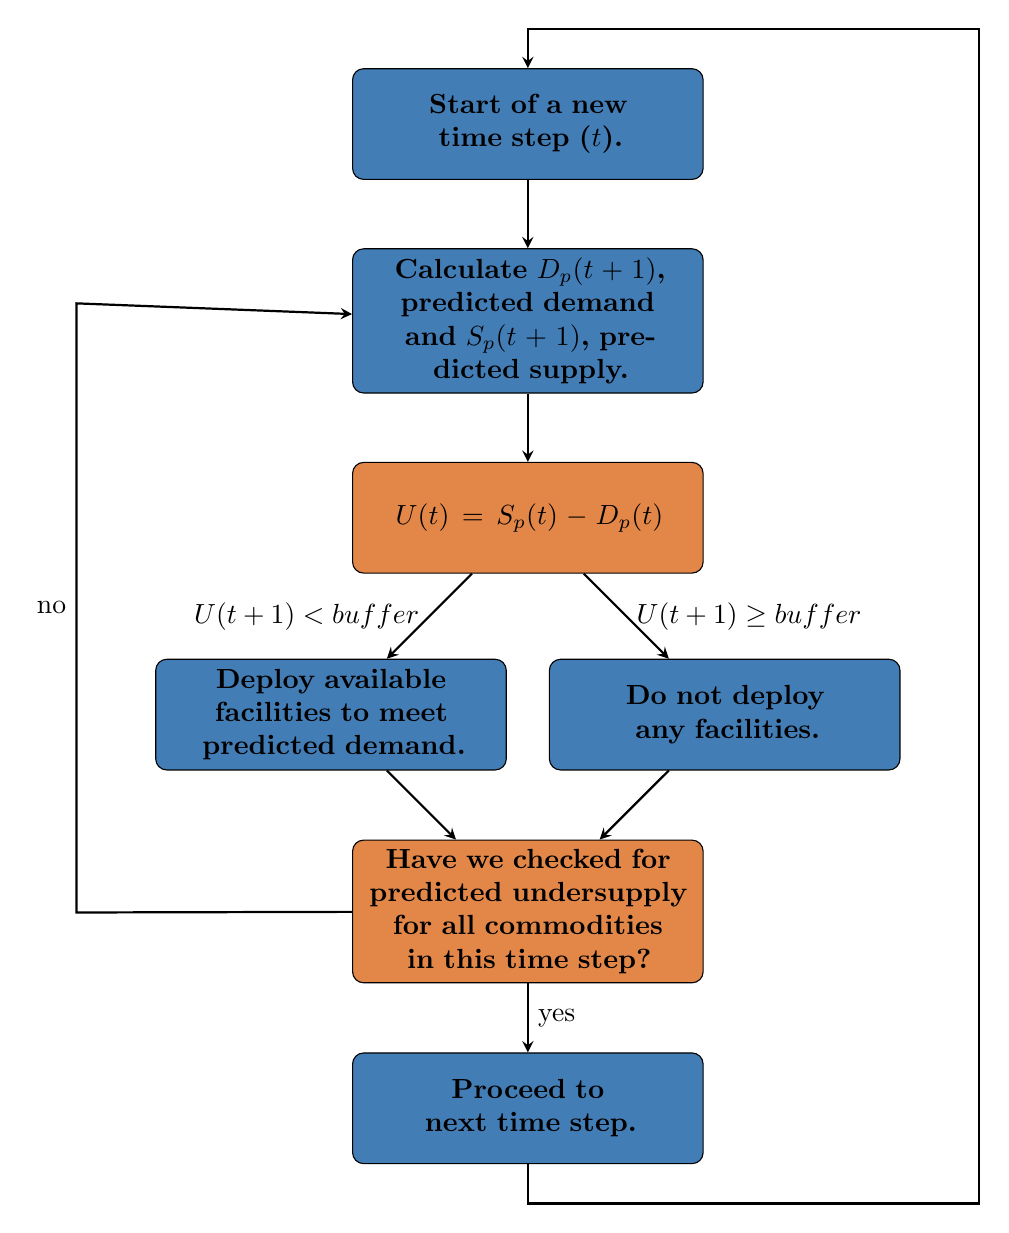
\begin{tikzpicture}[node distance=2.5cm]
	\node (Start) [bblock] {\textbf{Start of a new time step ($t$).}};
	\node (Predict) [bblock, below of=Start] {\textbf{Calculate $D_p(t+1)$, predicted demand and $S_p(t+1)$, predicted supply.}};
	\node (IsThere) [oblock, below of=Predict]{\textbf{$U(t) = S_p(t)-D_p(t)$}};
	\node (Deploy) [bblock, below of=IsThere, xshift = -2.5cm]{\textbf{Deploy available facilities to meet predicted demand.} };
    \node (NoDeploy) [bblock, right of=Deploy, xshift = 2.5cm]{\textbf{Do not deploy any facilities.} };
    \node (All) [oblock, below of=Deploy, xshift = 2.5cm] {\textbf{Have we checked for predicted undersupply for all commodities in this time step?}};
    \node (End) [bblock, below of=All] {\textbf{Proceed to next time step.}};
	
	\draw [arrow] (Start) -- (Predict); 
	\draw [arrow] (Predict) -- (IsThere);
    \draw [arrow] (IsThere) -- node[anchor=east] {$U(t+1) < buffer$} (Deploy);
    \draw [arrow] (IsThere) -- node[anchor=west] {$U(t+1) \geq buffer$} (NoDeploy);
    \draw [arrow] (Deploy) -- (All);
    \draw [arrow] (NoDeploy) -- (All);
    \draw [arrow] (All) -- node[anchor=west] {yes} (End);
    \draw [arrow] (All) -- ([shift={(-3.5cm,0.9cm)}]All.south west)-- node[anchor=east] {no} ([shift={(-3.5cm,-0.7cm)}]Predict.north west)--(Predict);
    \draw [arrow] (End) |-([shift={(3.5cm,-0.5cm)}]End.south east)-- ([shift={(3.5cm,0.5cm)}]Start.north east)-|(Start);
    \end{tikzpicture}
	\caption{\Deploy logic flow at each time step in \Cyclus. }
	\label{fig:flow}
\end{figure*}

Where \deploy predicts an undersupply, it responds by deploying 
the fewest number of available facilities to meet demand with minimal 
oversupply.  

\subsection{\textbf{Basic User-Defined Input Variables}}
The user inputs specific variables to customize their
simulation. 
Descriptions of each input variable are found in the 
README of the \deploy github repository \cite{d3ploy_doi_2019}.

Essentially, the user must define the facilities the 
\deploy institution controls and can deploy. 
The user must also define the driving commodity, all facility capacities 
for producing that commodity, its demand 
equation, and which method predicts supply and demand. 
For example, the user can define a demand equation for power of 
$1000 \times timestep$ MW and \deploy will deploy available reactor and supporting 
facilities to meet the defined power demand. 

The user can also provide a time-dependent equation that governs
preference for a particular facility compared to other facilities that 
provide the same commodity. 
For example, the user can define a \gls{LWR} and a \gls{SFR} to have
preferences of $101 - timestep$ and $timestep$ respectively. 
The institution will prefer deployment of \gls{LWR} facilities over 
\gls{SFR} before time step 51. 

The user can constrain facility deployment 
until a sizable inventory of a specific commodity is accumulated.  
The user can also define an initial facility list of facilities that 
are present in the institution at the beginning of the simulation. 

\subsection{\textbf{Prediction Algorithms}}
Three interchangeable algorithm classes govern demand and supply 
predictions: non-optimizing, deterministic optimizing, and stochastic
optimizing. 

Three methods were implemented in the non-optimizing class: 
moving average (MA),
autoregressive moving average (ARMA), and autoregressive 
conditional heteroskedasticity (ARCH).
Four methods were implemented in the deterministic optimizing class: 
Polynomial fit regression, simple exponential smoothing,  
triple exponential smoothing (holt-winters), and fast fourier 
transform (fft). 
One method was implemented for stochastic optimizing model: 
stepwise seasonal.  

The user can choose which prediction algorithm governs each
\deploy facility. 
The effectiveness of a prediction algorithm depends on the type 
of power demand in a scenario and the type of commodity (demand 
driving commodity vs non-driving commodity, demand driven 
deployment vs supply driven deployment etc.). 
For example, the most effective method
for predicting demand and supply for the power commodity in a scenario  
with a sinusoidal power demand is the triple exponential smoothing method. 
However, for the non-driving commodities in the same 
scenario, the fast fourier transform method is more effective than triple 
exponential smoothing. 
This paper will comment on these categories of problems and their suitable
algorithms. 

\begin{table*}[!htb]
    \centering
    \caption {Transition scenario parameters that are consisted for constant, linear increasing and sinusoidal power demand simulations}
	\label{tab:transition-scenario-all}
    \begin{tabular}{|l|p{4.5cm}|}
    \hline
    \textbf{Parameters}    & \textbf{Description} \\ \hline
    Facilities Present     & \texttt{Source} (Capacity: 3000kg), \texttt{Reactor} (Capacity: 1000MW), \texttt{Sink} (Capacity: 50000kg)      \\ \hline
    New Reactor Parameters & Cycle time: 18, Refuel time: 1\\ \hline
    Driving Commodity & Power \\ \hline
    \end{tabular}
\end{table*}

\begin{table*}[!htb]
    \centering
    \caption {Constant Power Demand Transition Scenario's Parameters}
	\label{tab:transition-scenario-constant-power}
    \begin{tabular}{|l|l|p{4.5cm}|}
    \hline
                                     & \textbf{Parameters}    & \textbf{Description} \\ \hline
    \textbf{Overall}& Demand Equation & 10000 MW \\ \hline
    \multirow{2}{*}{\textbf{Power Commodity}} & Prediction Method      &  Fast Fourier Transform\\ \cline{2-3} 
                                     & Supply Buffer          &  3000 MW (3 reactor capacities)\\ \hline
    \multirow{2}{*}{\textbf{Fuel Commodity}}  & Prediction Method      &  Moving Average\\ \cline{2-3}
                                     & Supply Buffer & 0 kg \\ \hline
    \multirow{2}{*}{\textbf{Spent Fuel Commodity}}  & Prediction Method      &  Moving Average\\ \cline{2-3}
                                     & Capacity Buffer & 0 kg \\ \hline
    \end{tabular}
\end{table*}

\subsection{\textbf{Demand-driven vs. Supply-driven Institutions}}
Within \deploy, there are two institutions: \texttt{Demand-}
\texttt{DrivenDeploymentInst} and \texttt{SupplyDrivenDeployment}. 
\texttt{Inst}. 
The prior is used for the front-end of the fuel cycle and the latter is used 
for the back-end. 
For example, for front end facilities, the reactor demands 
fuel and \texttt{DemandDrivenDeploymentInst} triggers the deployment 
of fuel fabrication facilities to create supply meeting the demand 
for fuel. 
For back end facilities, the reactor generates spent fuel 
and \texttt{SupplyDrivenDeploymentInst} triggers the deployment of 
waste repository facilities to create capacity for storage of the supply 
of spent fuel. 

\subsection{\textbf{Installed Capacity}}
The user can choose between deploying facilities based on the difference 
between predicted demand and predicted supply or predicted demand and 
installed capacity. 
There are two advantages to use installed capacity over predicted 
supply. 
The first is for facilities that provide intermittent supply, such as a 
reactor facility that has a designated refueling time. 
During time steps in which a reactor is refueling, the user might not 
want \deploy to deploy more facilities to make up for the lack of supply
caused by this one time step gap in supply. 
The second is for situations where the input commodity for a facility has
run out and the facility that produces the input commodity 
is no longer commissionable. 
Therefore, with the demand for the output commodity of that facility, \deploy
would deploy that facility to meet the demand, however due to the lack of 
the input commodity, even if there are infinite numbers of that facility, 
it will not produce the output commodity. 
For example, in a transition scenario from LWRs to fast reactors, the fast 
reactor demand for Pu may exceed the inventory provided by LWRs before 
they were decommissioned. 
This will result in the deployment of mixer facilities that generate the 
fast reactor fuel despite the lack of plutonium to generate the fuel. 
This can be avoided by constraining fast reactor facility deployment 
until a sizable inventory of Pu is accumulated. 

\subsection{\textbf{Supply/Capacity Buffer}}
In \texttt{DemandDrivenDeploymentInst}, the user can choose to provide a
buffer for predicted supply.
\Deploy will deploy facilities to meet the predicted demand with the 
additional buffer. 

In \texttt{SupplyDrivenDeploymentInst}, the user can choose to 
provide a buffer for predicted capacity.
\Deploy will deploy facilities to meet the predicted supply with the 
additional buffer. 
The buffer can be defined as a percentage value (equation \ref{eq:perc}) 
or an absolute value (equation \ref{eq:abs}).  

\begin{equation}
    \label{eq:perc}
    S_{pwb} = S_{p}*(1+d)
\end{equation}
\begin{equation}
    \label{eq:abs}
    S_{pwb} = S_{p}+a
\end{equation}
where $S_{pwb}$ is predicted supply/capacity with buffer, 
$S_p$ is the predicted supply/capacity without buffer, 
$d$ is the percentage value in decimal form, 
and $a$ is the absolute value of the buffer. 

%%%%%%%%%%%%%%%%%%%%%%%%%%%%%%%%%%%%%%%%%%%%%%%%%%%%%%%%%%%%%%%%%%%%
\section{Demonstration of d3ploy capabilities}
Constant, linearly increasing, and sinusoidal power demand simulations
are shown to demonstrate \deploy's capabilities. 
A balance between the various system parameters must be 
met for each type of simulation to meet the goal of 
minimizing undersupply and under capacity for the various 
commodities. 
The input files and scripts to produce the plots in this paper 
can be reproduced using \cite{d3ploy_doi_2019}. 

These simulations are basic transition scenarios that only include
three types of facilities: \texttt{source}, \texttt{reactor} and 
\texttt{sink}.
All simulations in this work begin with a ten reactor facilities, 
\texttt{reactor1} to \texttt{reactor10}. 
These reactors have staggered cycle lengths and lifetimes 
so that they do not all refuel and decommission at the same time 
steps. 
When the ten initial reactor facilities begin to decommission, 
\deploy deploys reactor facilities of \texttt{newreactor} type
to meet unmet demand for power. 
All the simulations deploy facilities based on the relationship
between predicted demand and installed capacity. 
This capability was discussed in the previous section.  
Table \ref{tab:transition-scenario-all} shows the simulation 
parameters that are consistent across all the discussed 
scenarios. 

These basic transition scenarios were set up to 
demonstrate \deploy's capabilities for simulating 
transition scenarios and 
to inform decisions about input parameters when setting up larger 
demand transition scenarios with many facilities. 

\subsection{\textbf{Transition Scenario: Constant Demand}}


\begin{figure*}[!htbp]
    \centering
    \begin{subfigure}[t]{\textwidth}
    \centering
        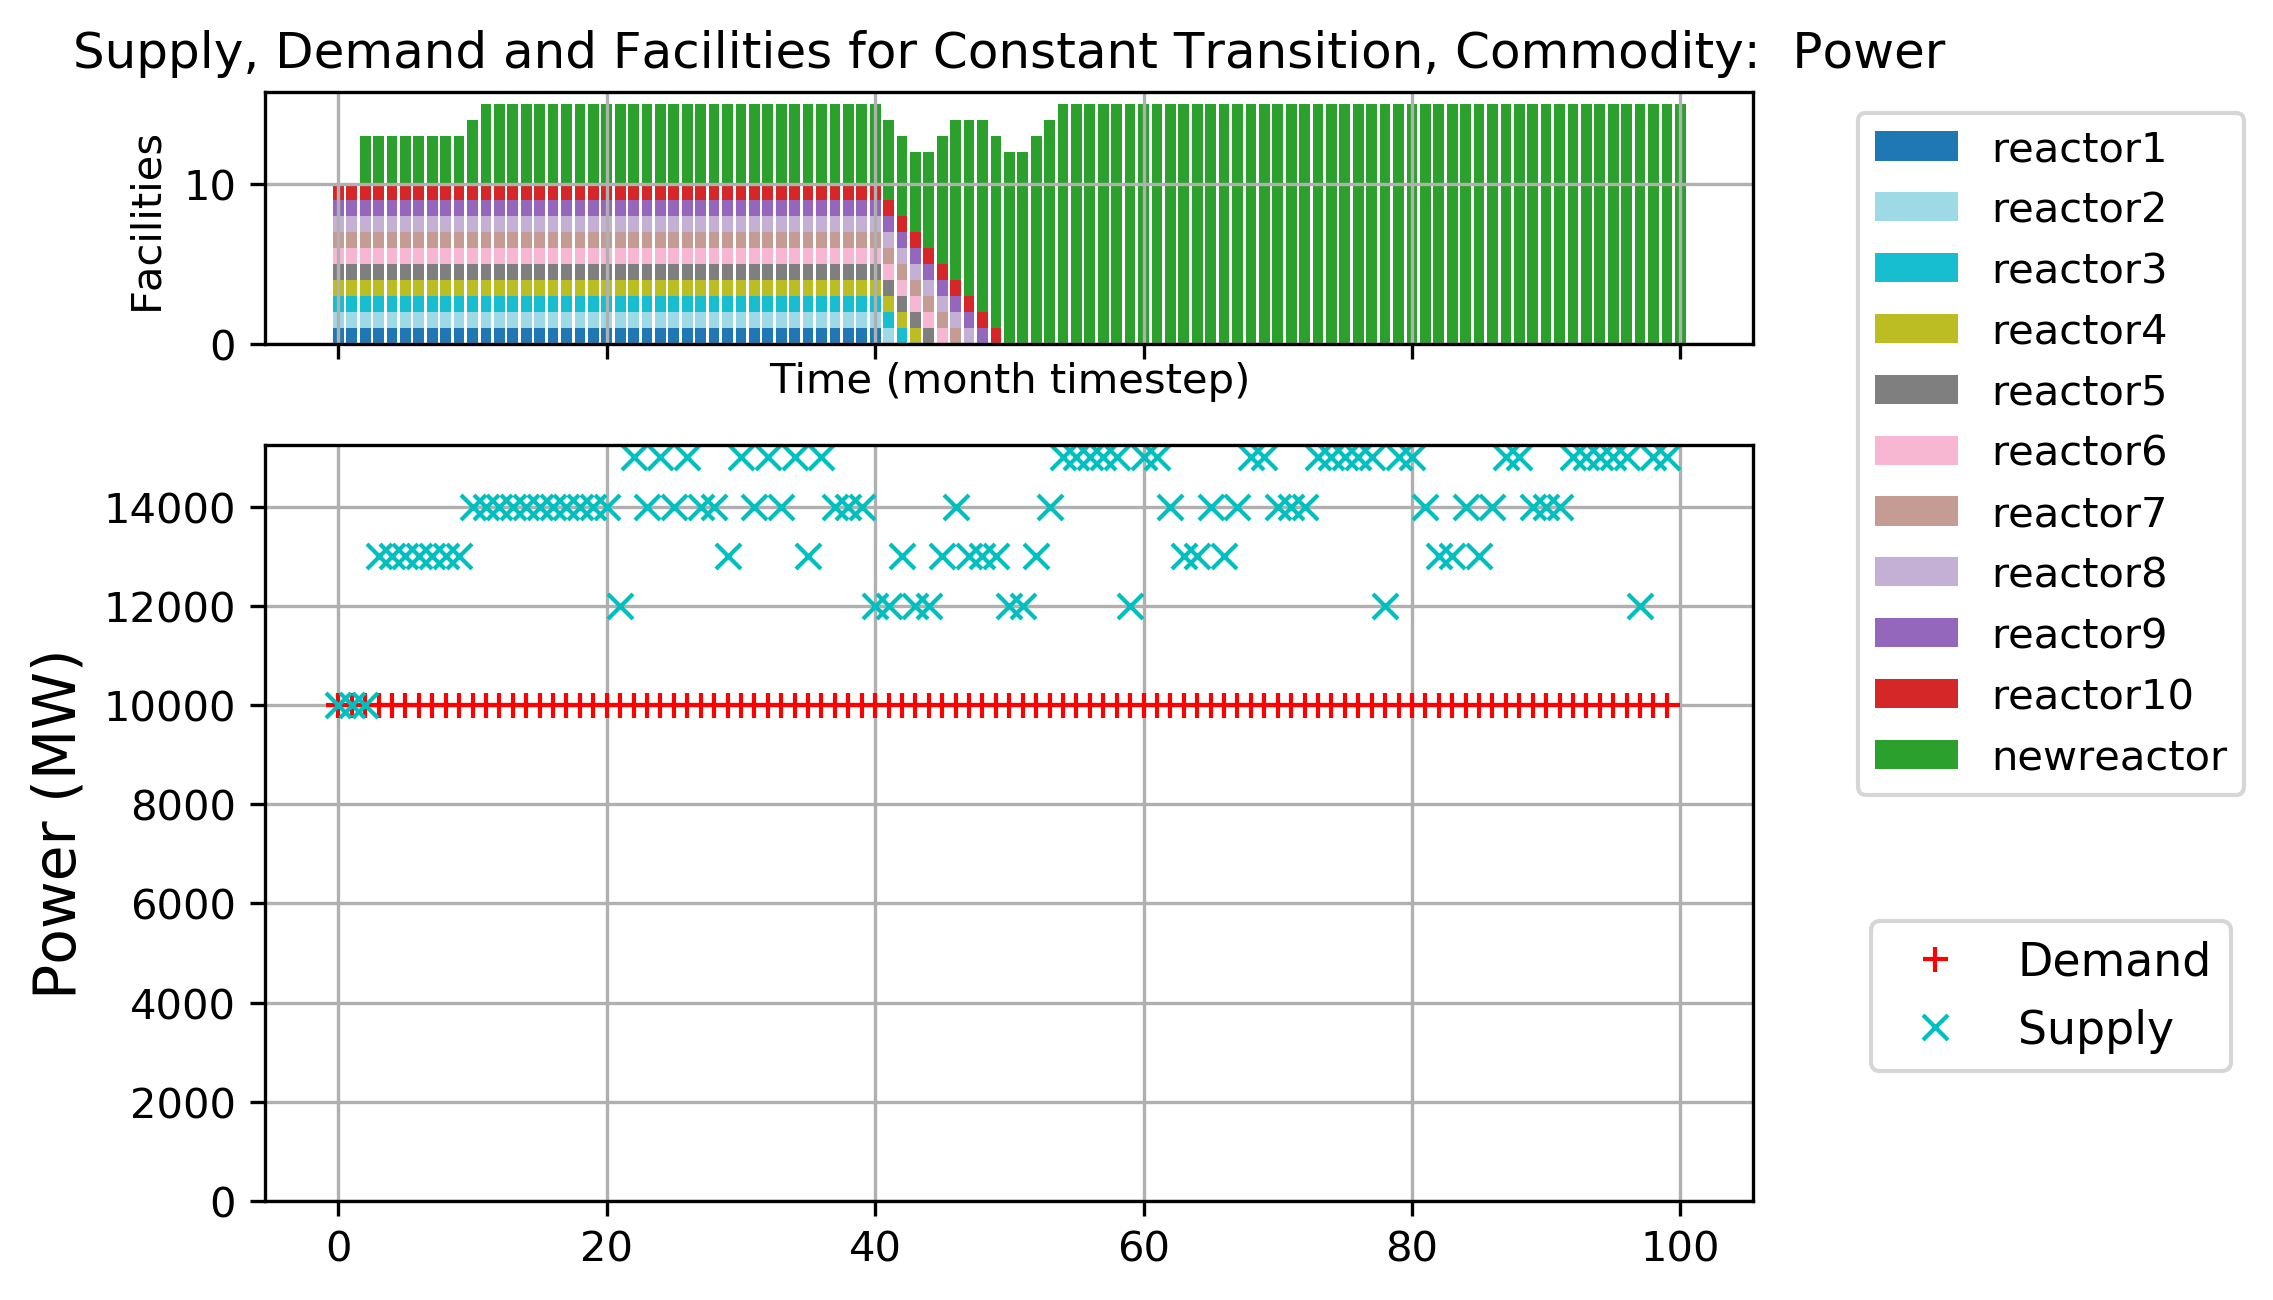
\includegraphics[width=0.8\linewidth]{figures/constanttransition-power.png} 
        \caption{The power demand is a user-defined equation and power is supplied by the reactors.}
        \label{fig:constanttransition-power}
    \end{subfigure}
    \begin{subfigure}[t]{0.65\textwidth}
        \centering
        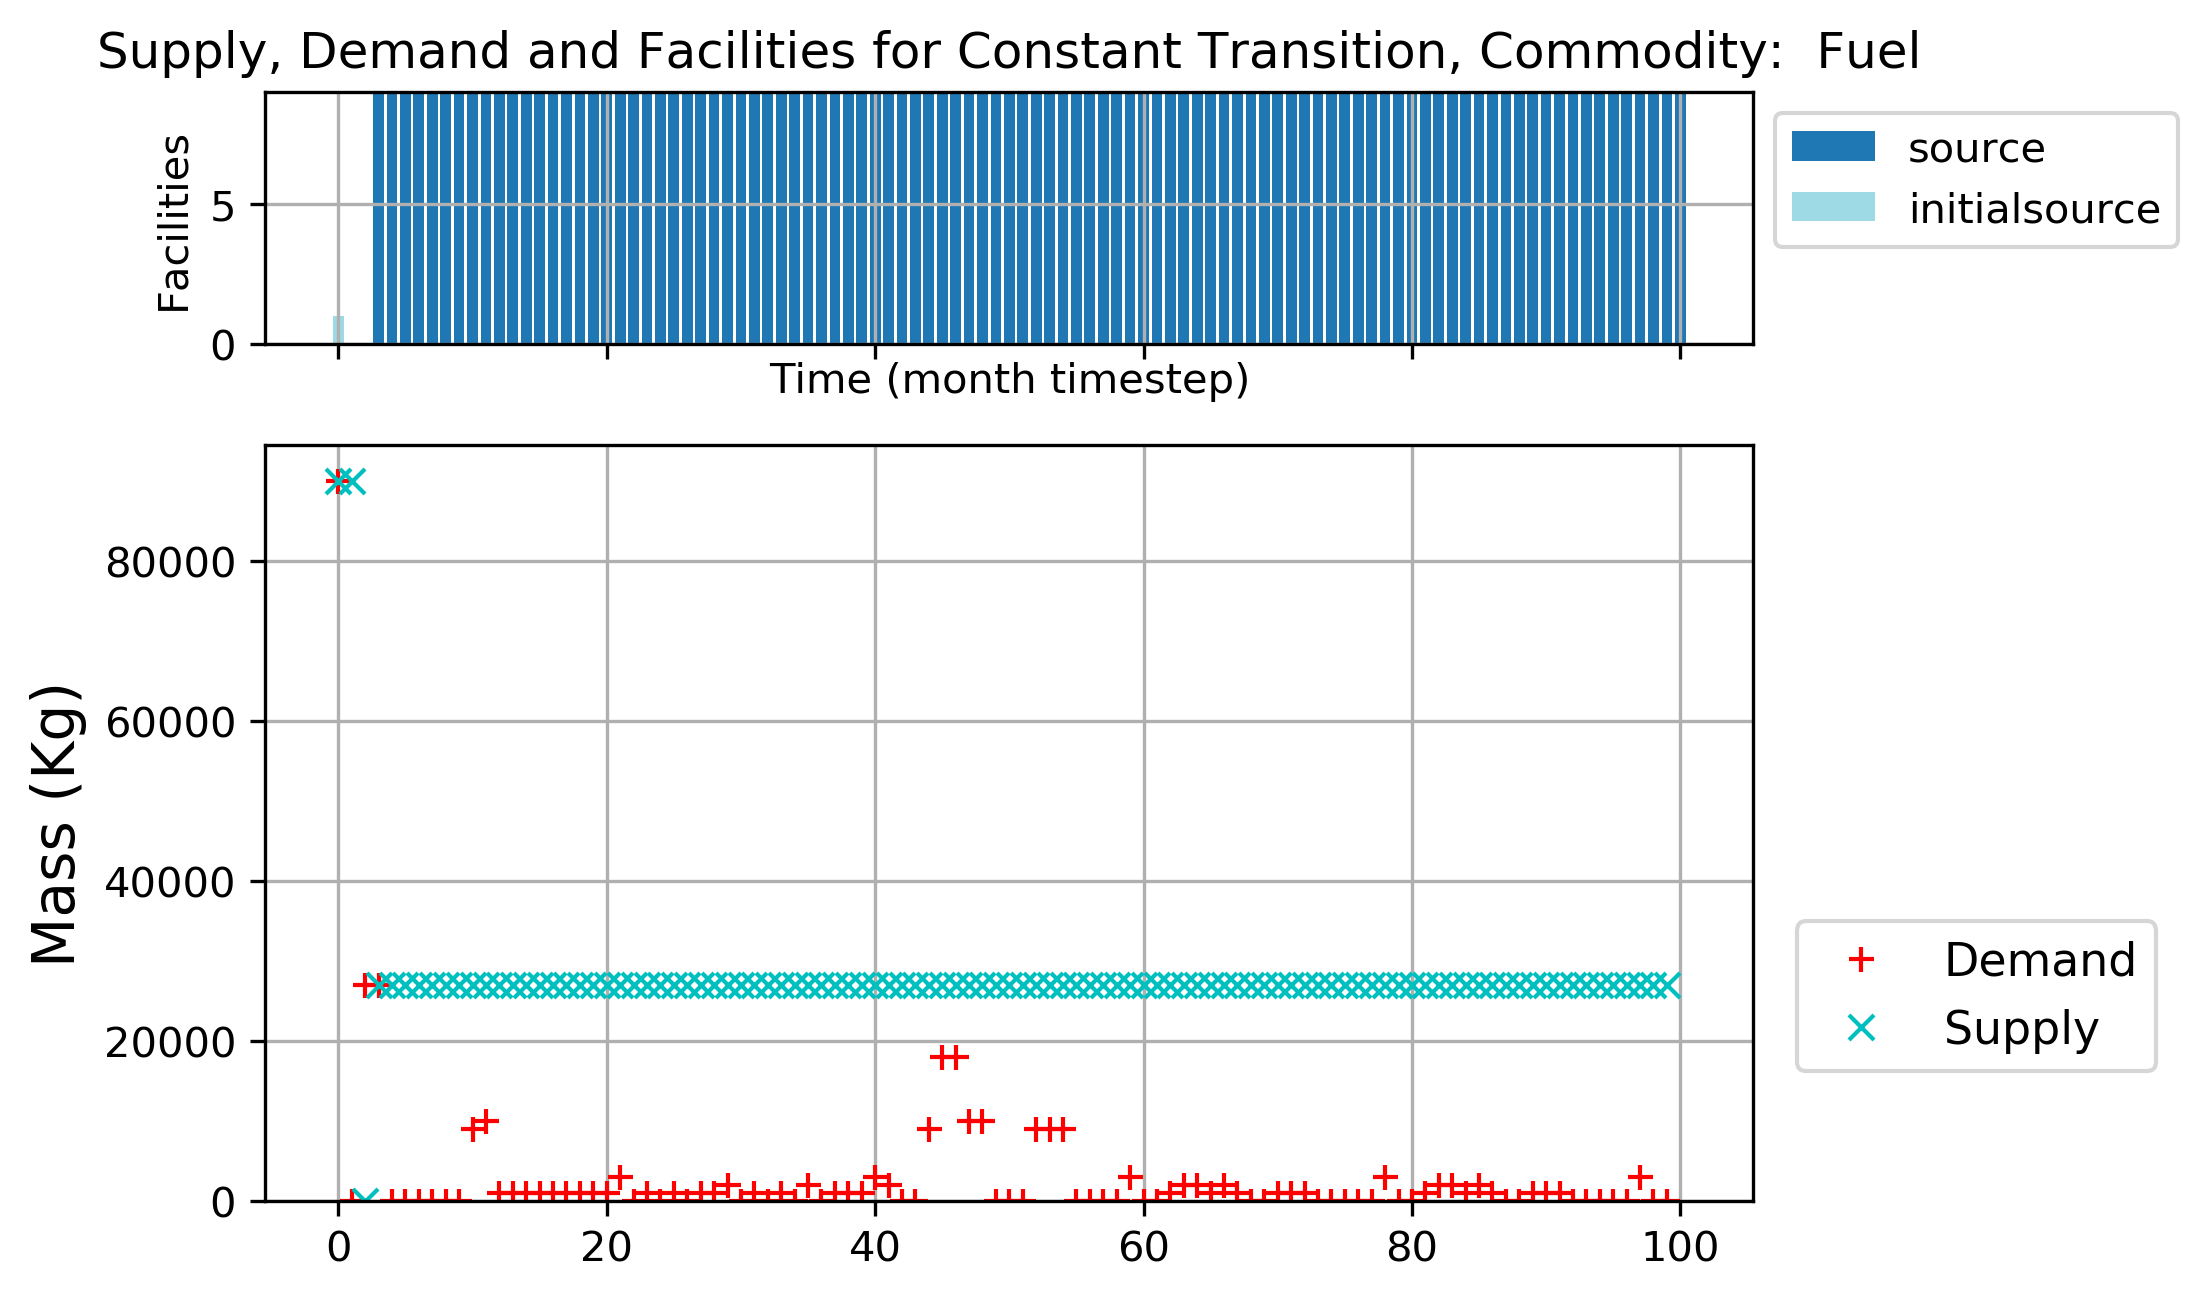
\includegraphics[width=\linewidth]{figures/constanttransition-fuel.png} 
        \caption{Fuel is demanded by reactors and supplied by source facilities.}
	    \label{fig:constanttransition-fuel}
    \end{subfigure}
    \begin{subfigure}[t]{0.65\textwidth}
        \centering
        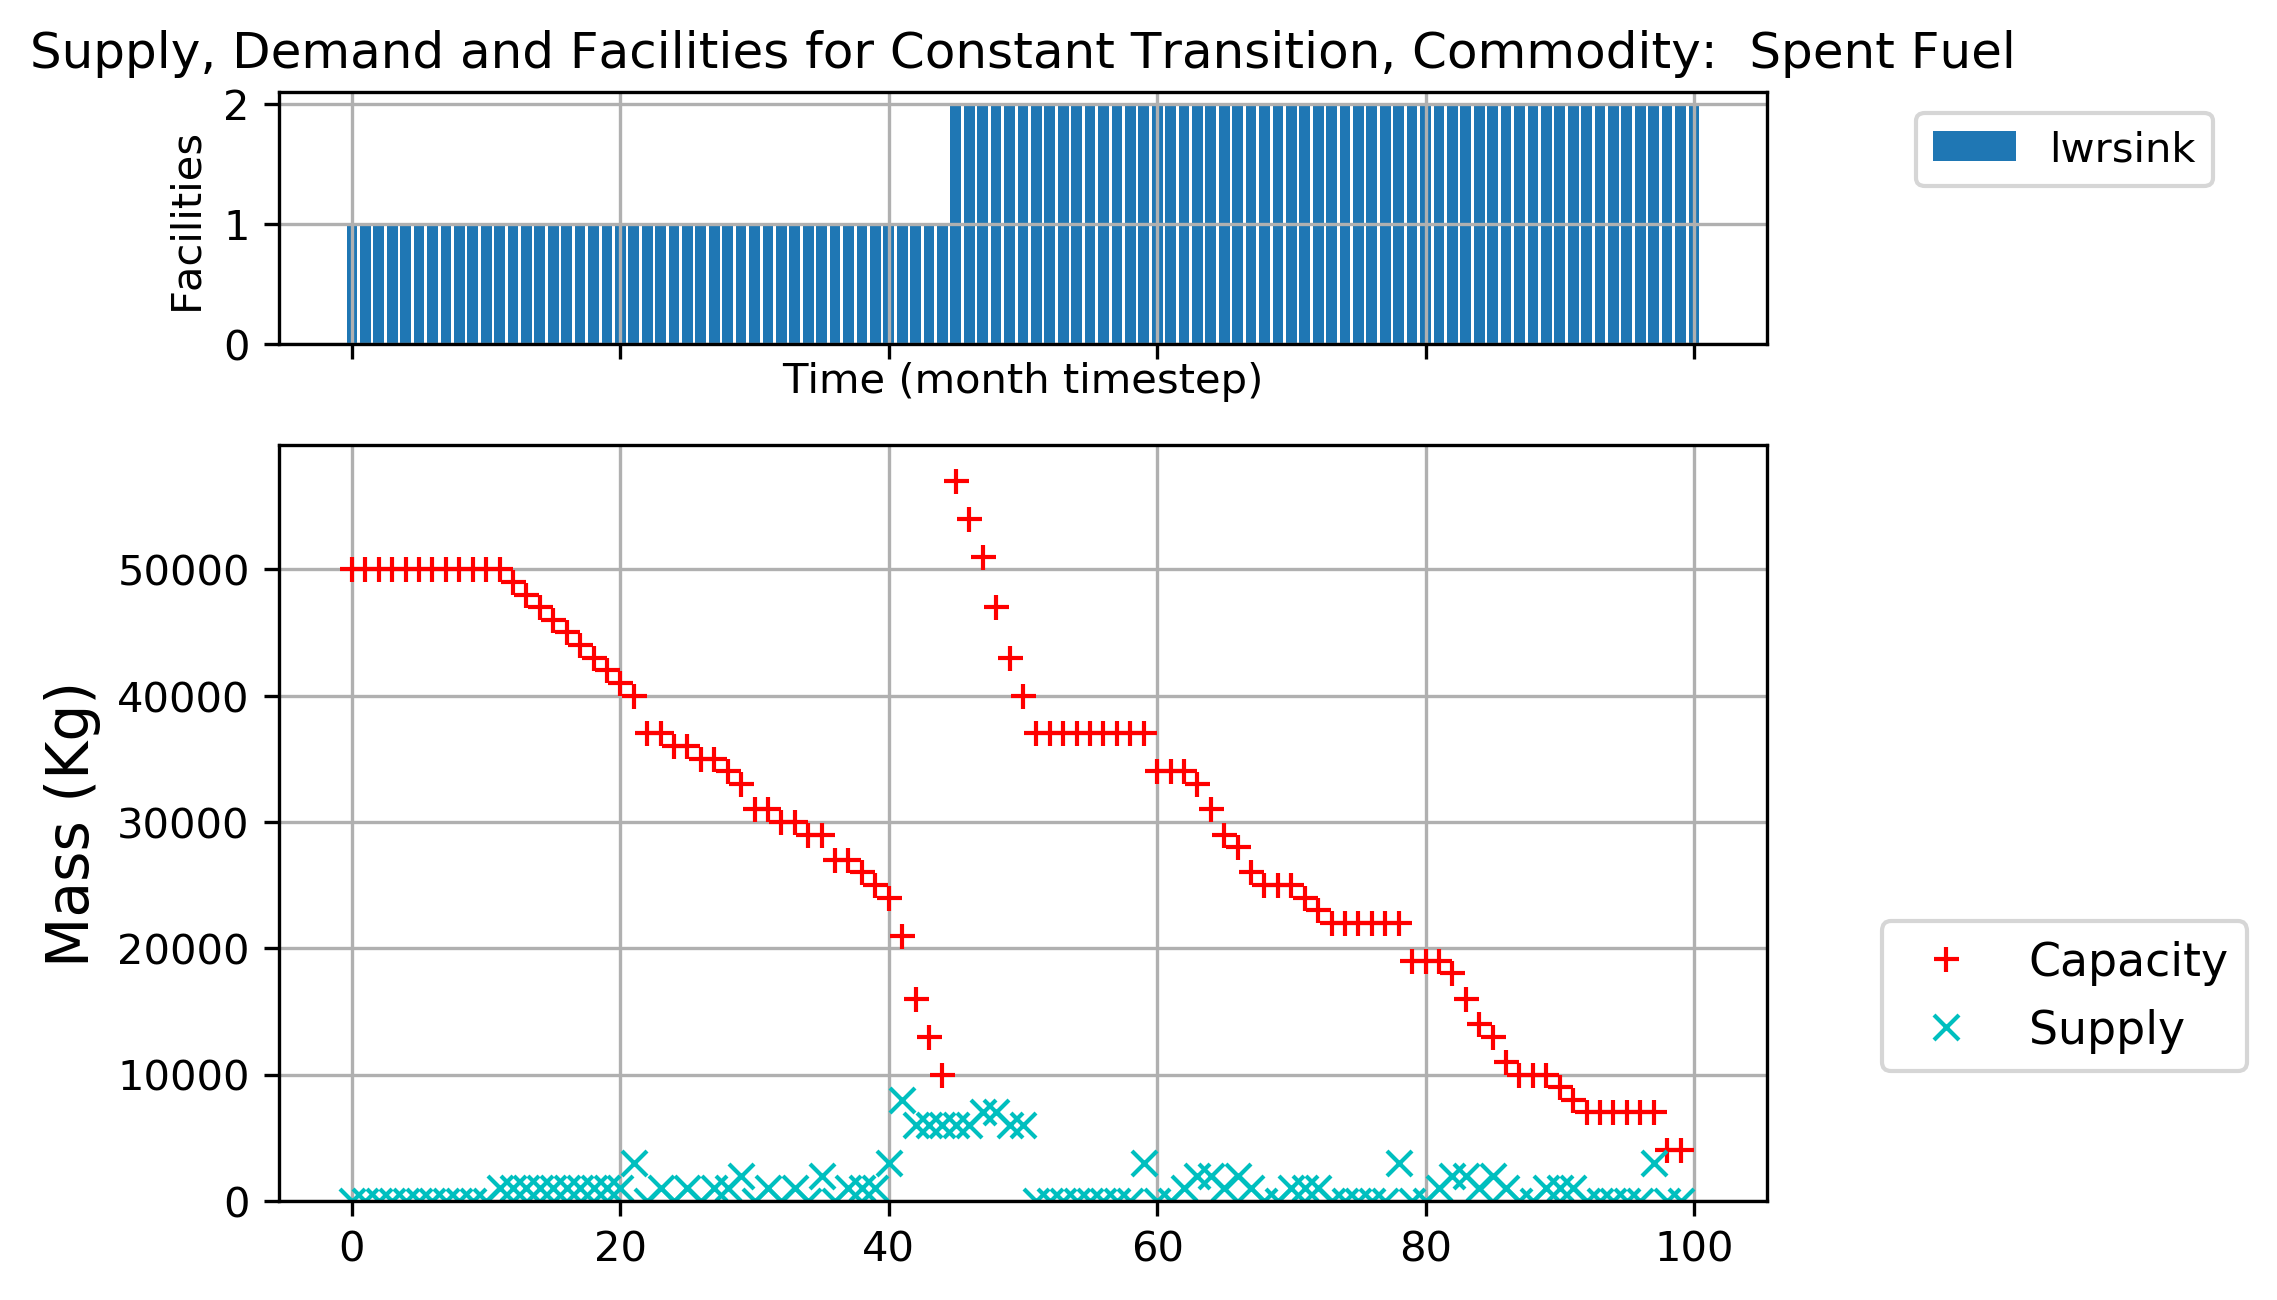
\includegraphics[width=\linewidth]{figures/constanttransition-spentfuel.png} 
        \caption{Spent Fuel is supplied by reactors and the capacity is provided by sink facilities.}
        \label{fig:constanttransition-spentfuel}
    \end{subfigure}
    \caption{Transition Scenario: Constant Power Demand of 10000MW}
\end{figure*}

\begin{table*}[htb]
    \centering
    \caption {Undersupply results for each commodity in each scenario}
	\label{tab:transition-scenario-results}
    \begin{tabular}{|l|l|p{4.5cm}|}
    \hline
    \textbf{Transition Scenario}    & \textbf{Commodity}    & \textbf{No. of time steps with undersupply} \\ \hline
    \multirow{2}{*}{\textbf{Constant Power}} & Fuel & 1 \\ \cline{2-3}
                                             & Power & 0 \\ \cline{2-3}
                                             & Spent Fuel & 0 \\ \hline
    \multirow{2}{*}{\textbf{Linearly Increasing Power}} & Fuel & 1 \\ \cline{2-3}
                                             & Power & 0 \\ \cline{2-3}
                                             & Spent Fuel & 0 \\ \hline
    \multirow{2}{*}{\textbf{Sinusoidal Power}} & Fuel & 1 \\ \cline{2-3}
                                             & Power & 1 \\ \cline{2-3}
                                             & Spent Fuel & 0 \\ \hline
    \end{tabular}
\end{table*}

\begin{table*}[!htbp]
    \centering
    \caption {Linearly Increasing Power Demand Transition Scenario's Parameters}
	\label{tab:transition-scenario-growing-power}
    \begin{tabular}{|l|l|p{4.5cm}|}
    \hline
                                     & \textbf{Parameters}    & \textbf{Description} \\ \hline
    \textbf{Overall}& Demand Equation & Time<40: 10000 MW, Time>40: 250*t MW \\ \hline
    \multirow{2}{*}{\textbf{Power Commodity}} & Prediction Method      &  Fast Fourier Transform \\ \cline{2-3} 
                                     & Supply Buffer          &  2000 MW (2 reactor capacities)\\ \hline
    \multirow{2}{*}{\textbf{Fuel Commodity}}  & Prediction Method      &  Moving Average\\ \cline{2-3}
                                     & Supply Buffer & 1000 kg \\ \hline
    \multirow{2}{*}{\textbf{Spent Fuel Commodity}}  & Prediction Method      &  Fast Fourier Transform \\ \cline{2-3}
                                     & Capacity Buffer & 0 kg \\ \hline
    \end{tabular}
\end{table*}

\begin{table*}[!htbp]
    \centering
    \caption {Sinusoidal Power Demand Transition Scenario's Parameters}
	\label{tab:transition-scenario-sine-power}
    \begin{tabular}{|l|l|p{4.5cm}|}
    \hline
                                     & \textbf{Parameters}    & \textbf{Description} \\ \hline
    \textbf{Overall}& Demand Equation & $1000sin(\frac{\pi*t}{3})+10000$ \\ \hline
    \multirow{2}{*}{\textbf{Power Commodity}} & Prediction Method      &  Triple Exponential Smoothing \\ \cline{2-3} 
                                     & Supply Buffer          &  2000 MW (2 reactor capacities)\\ \hline
    \multirow{2}{*}{\textbf{Fuel Commodity}}  & Prediction Method      &  Moving Average\\ \cline{2-3}
                                     & Supply Buffer & 1000 kg \\ \hline
    \multirow{2}{*}{\textbf{Spent Fuel Commodity}}  & Prediction Method      & Fast Fourier Transform\\ \cline{2-3}
                                     & Capacity Buffer & 0 kg \\ \hline
    \end{tabular}
\end{table*}

In this section, a constant power transition scenario is shown. 
Table \ref{tab:transition-scenario-constant-power} shows the 
simulation parameters used in this transition scenario. 

Figures \ref{fig:constanttransition-power}, \ref{fig:constanttransition-fuel}
and \ref{fig:constanttransition-spentfuel} demonstrate \deploy's capability 
to deploy reactor and supporting facilities to meet the user 
determined power demand and subsequently demanded secondary commodities 
with minimal undersupply. 
Table \ref{tab:transition-scenario-results} shows the number of 
undersupplied timesteps. 
In figure \ref{fig:constanttransition-power}, there are no time steps
in which the supply of power falls under demand.
By using a combination of the fast fourier transform method for predicting 
demand and setting the supply buffer to 3000MW (the capacity of 3 reactors), 
the user minimizes the number of undersupplied time steps of every commodity. 
To ensure there is no undersupply, it is important to perform a
sensitivity analysis of the size 
of buffer to use for each commodity. 

In figure \ref{fig:constanttransition-fuel},
a facility with a large fuel throughput is initially
deployed to meet the large initial fuel demand for the starting
up of ten reactors. 
\Deploy is prevented from deploying many supporting
facilities that end up being redundant at the later parts of 
the simulation, by having an initial facility with a large throughput
exist for the first few time steps in the simulation.
This is a reflection of reality in which reactor manufacturers will 
accumulate an appropriate amount of fuel inventory before starting 
up reactors. 
There is one time step where there is an undersupply after the 
decommissioning of the large initial facility.  
This is unavoidable since the prediction methods in \deploy are 
unable to predict this sudden drop in demand. 


\subsection{\textbf{Transition Scenario: Linearly Increasing Demand}}

\begin{figure*}[!htbp]
    \centering
    \begin{subfigure}[t]{\textwidth}
    \centering
        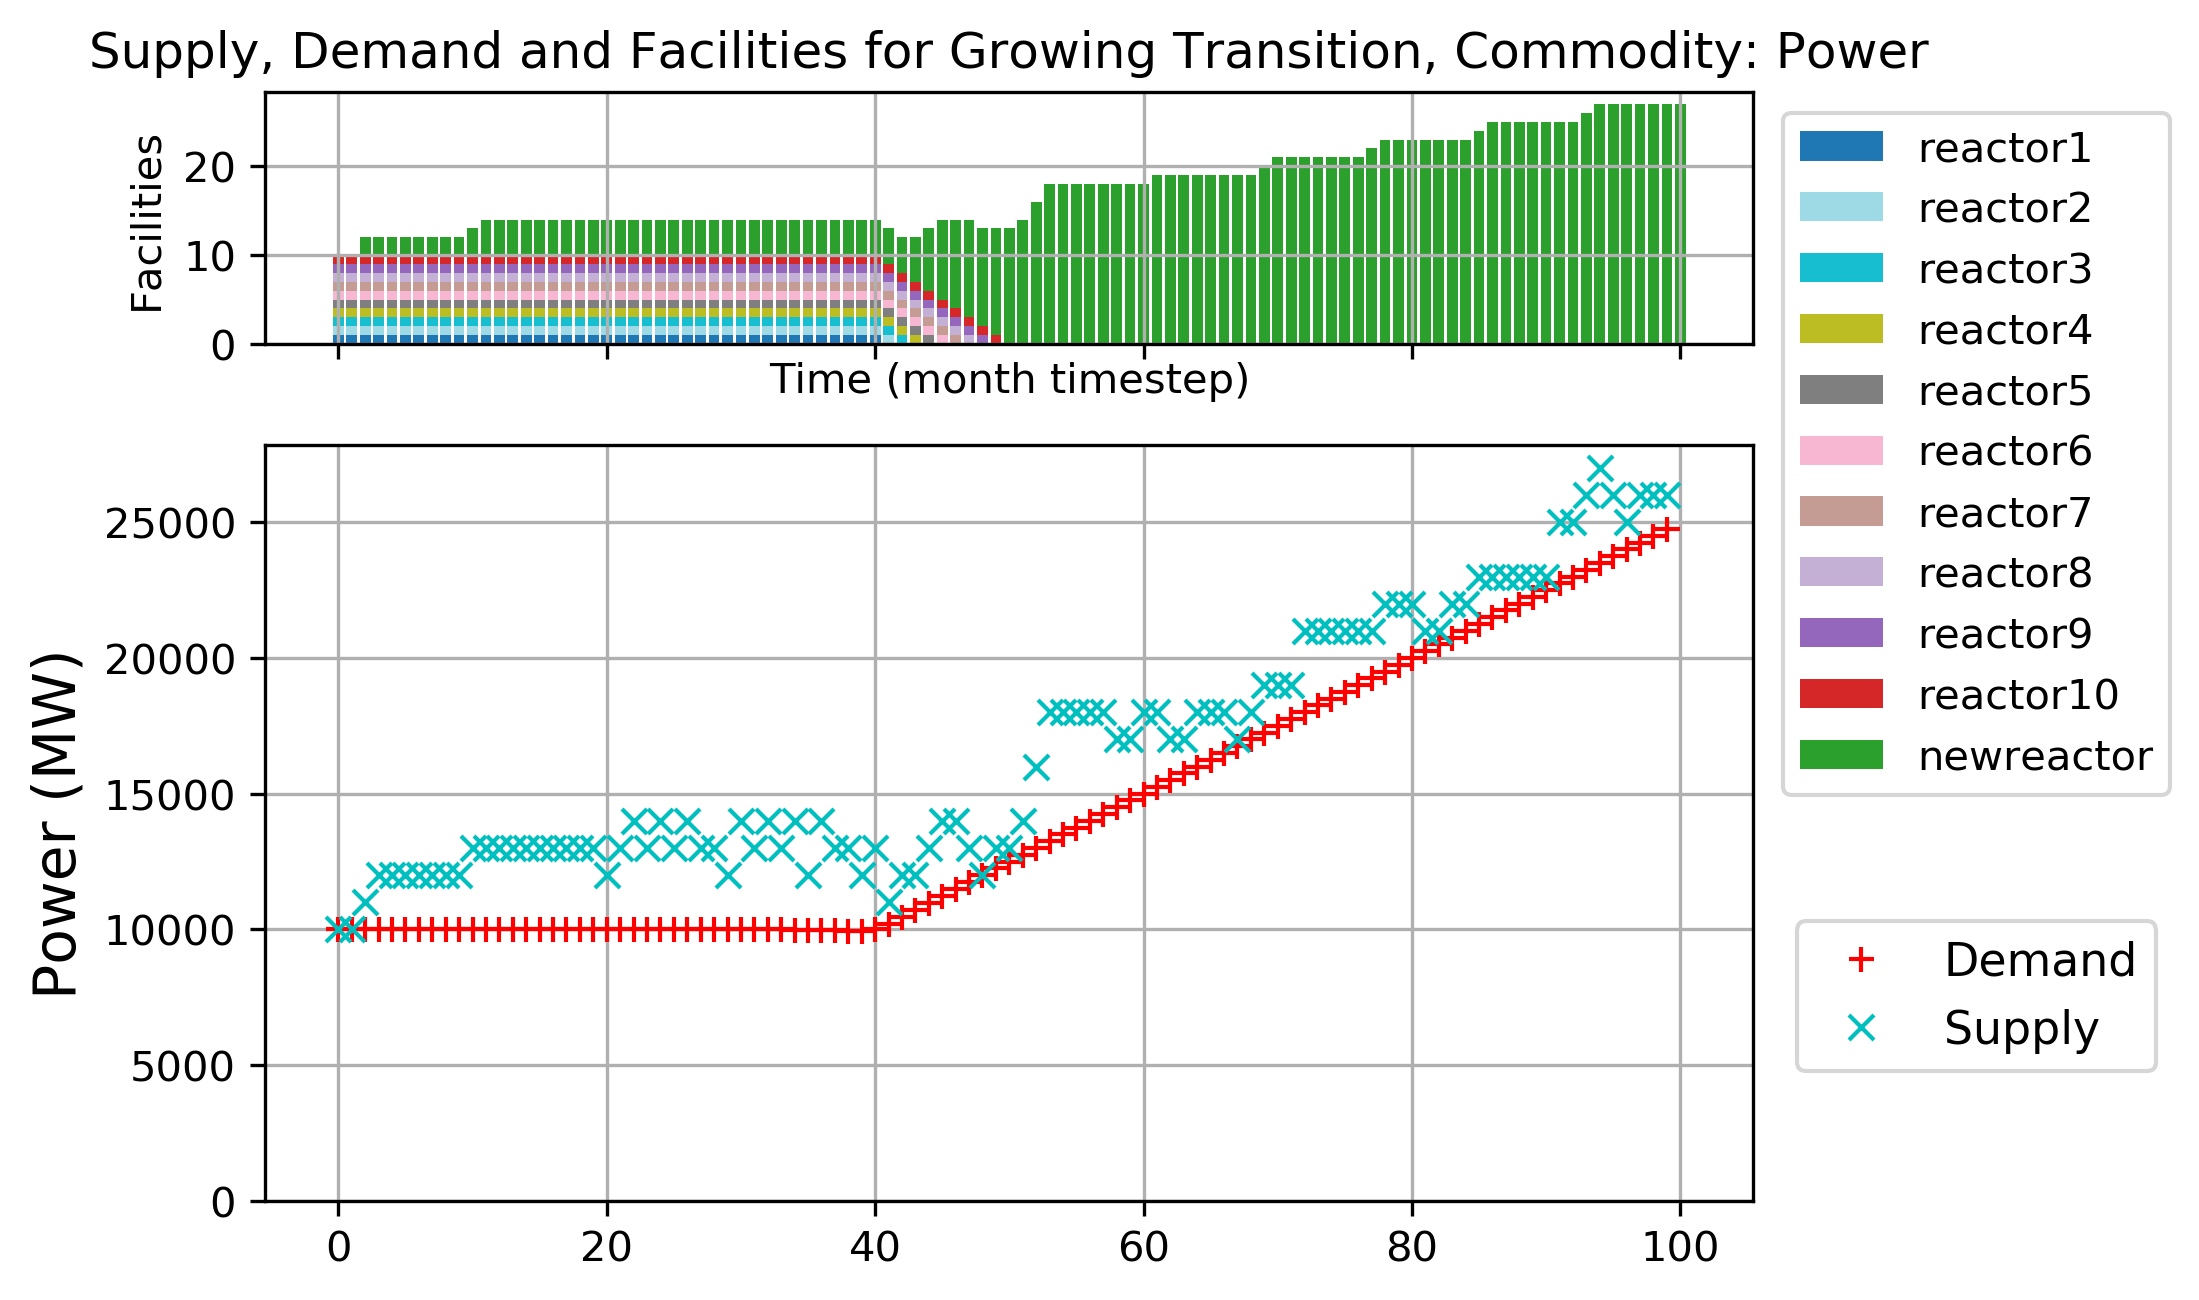
\includegraphics[width=0.8\linewidth]{figures/growingtransition-power.png} 
        \caption{The power demand is a user-defined equation and power is supplied by the reactors.}
        \label{fig:growingtransition-power}
    \end{subfigure}
    \begin{subfigure}[t]{0.65\textwidth}
        \centering
        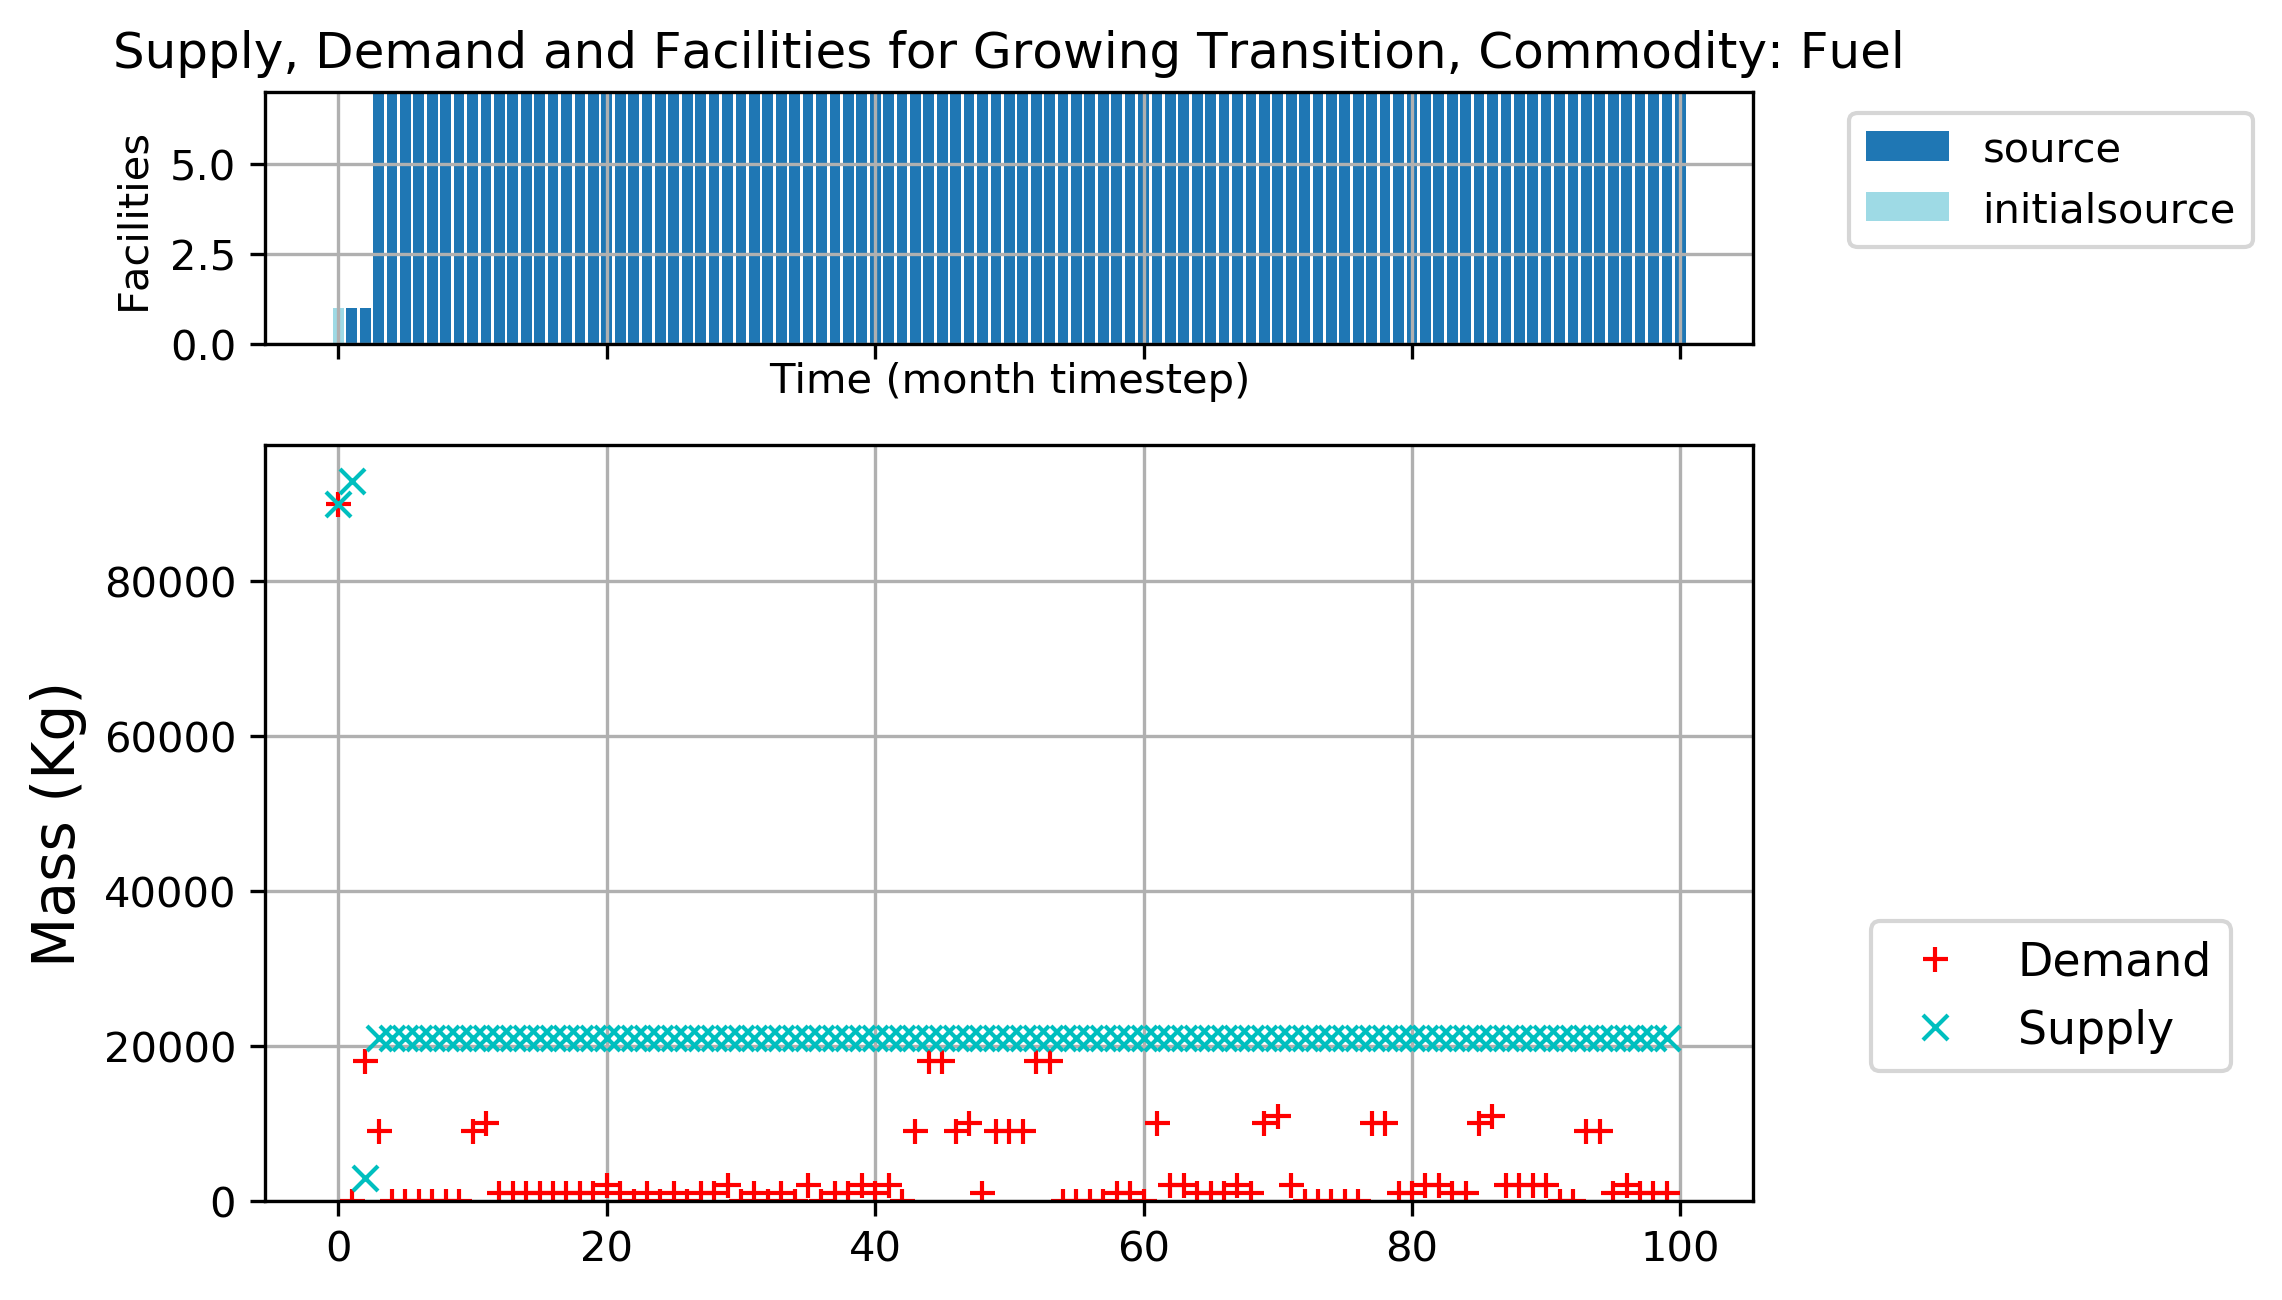
\includegraphics[width=\linewidth]{figures/growingtransition-fuel.png} 
        \caption{Fuel is demanded by reactors and supplied by source facilities.}
	    \label{fig:growingtransition-fuel}
    \end{subfigure}
    \begin{subfigure}[t]{0.65\textwidth}
        \centering
        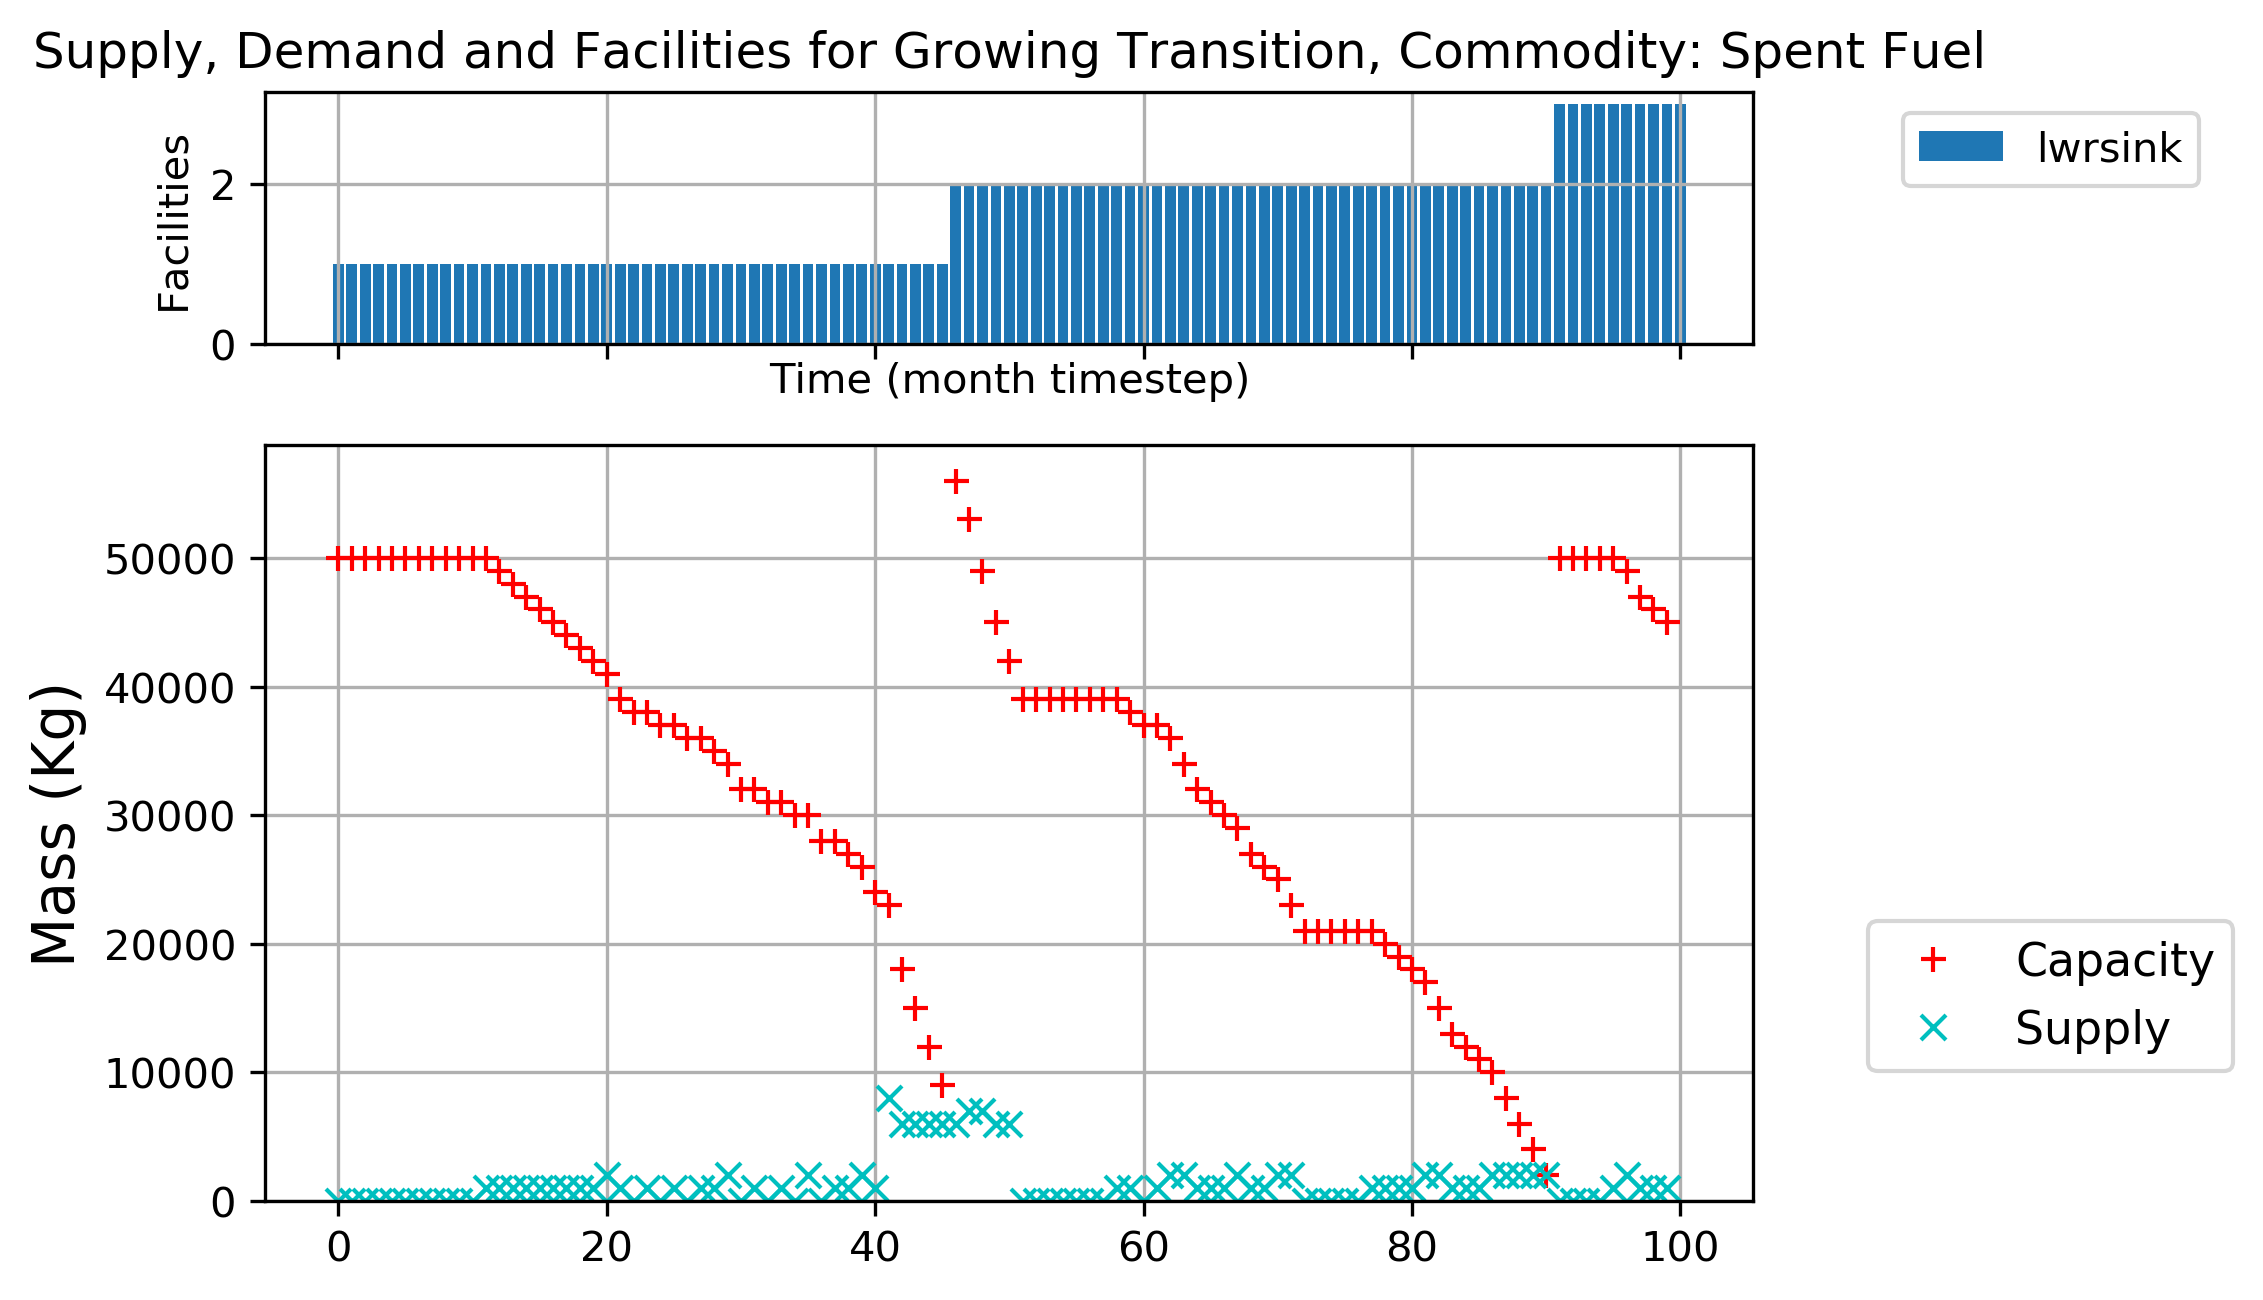
\includegraphics[width=\linewidth]{figures/growingtransition-spentfuel.png} 
        \caption{Spent Fuel is supplied by reactors and the capacity is provided by sink facilities.}
        \label{fig:growingtransition-spentfuel}
    \end{subfigure}
    \caption{Transition Scenario: Linearly increasing power demand.}
\end{figure*}

\begin{figure*}[!htbp]
    \centering
    \begin{subfigure}[t]{\textwidth}
    \centering
        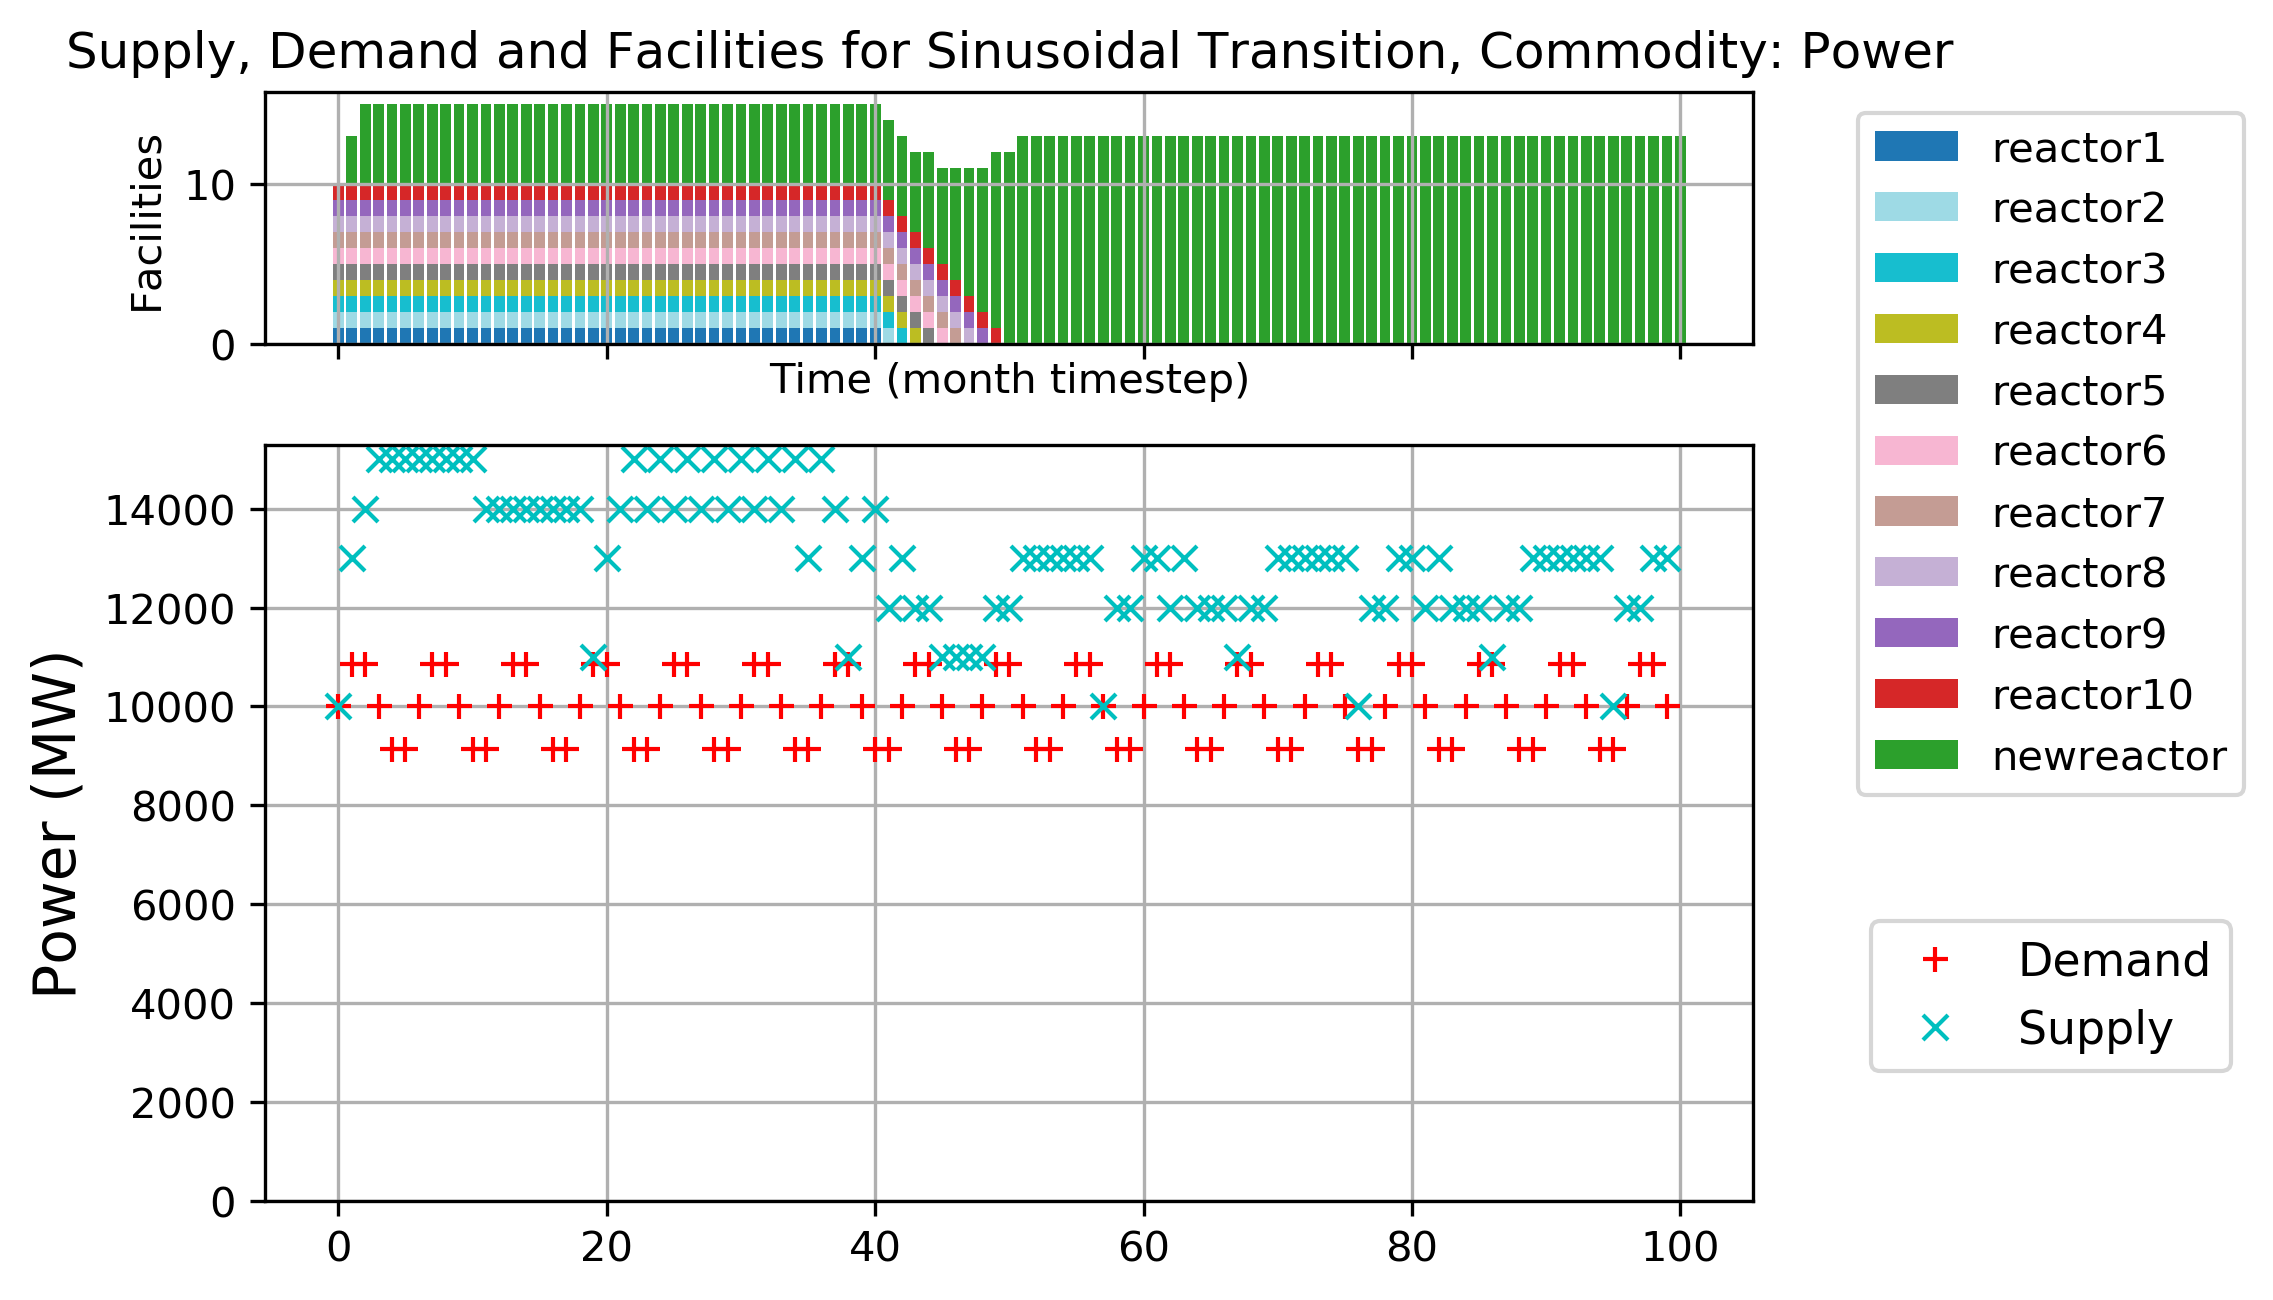
\includegraphics[width=0.8\linewidth]{figures/sinetransition-power.png} 
        \caption{The power demand is a user-defined equation and power is supplied by the reactors.}
        \label{fig:sinetransition-power}
    \end{subfigure}
    \begin{subfigure}[t]{0.65\textwidth}
        \centering
        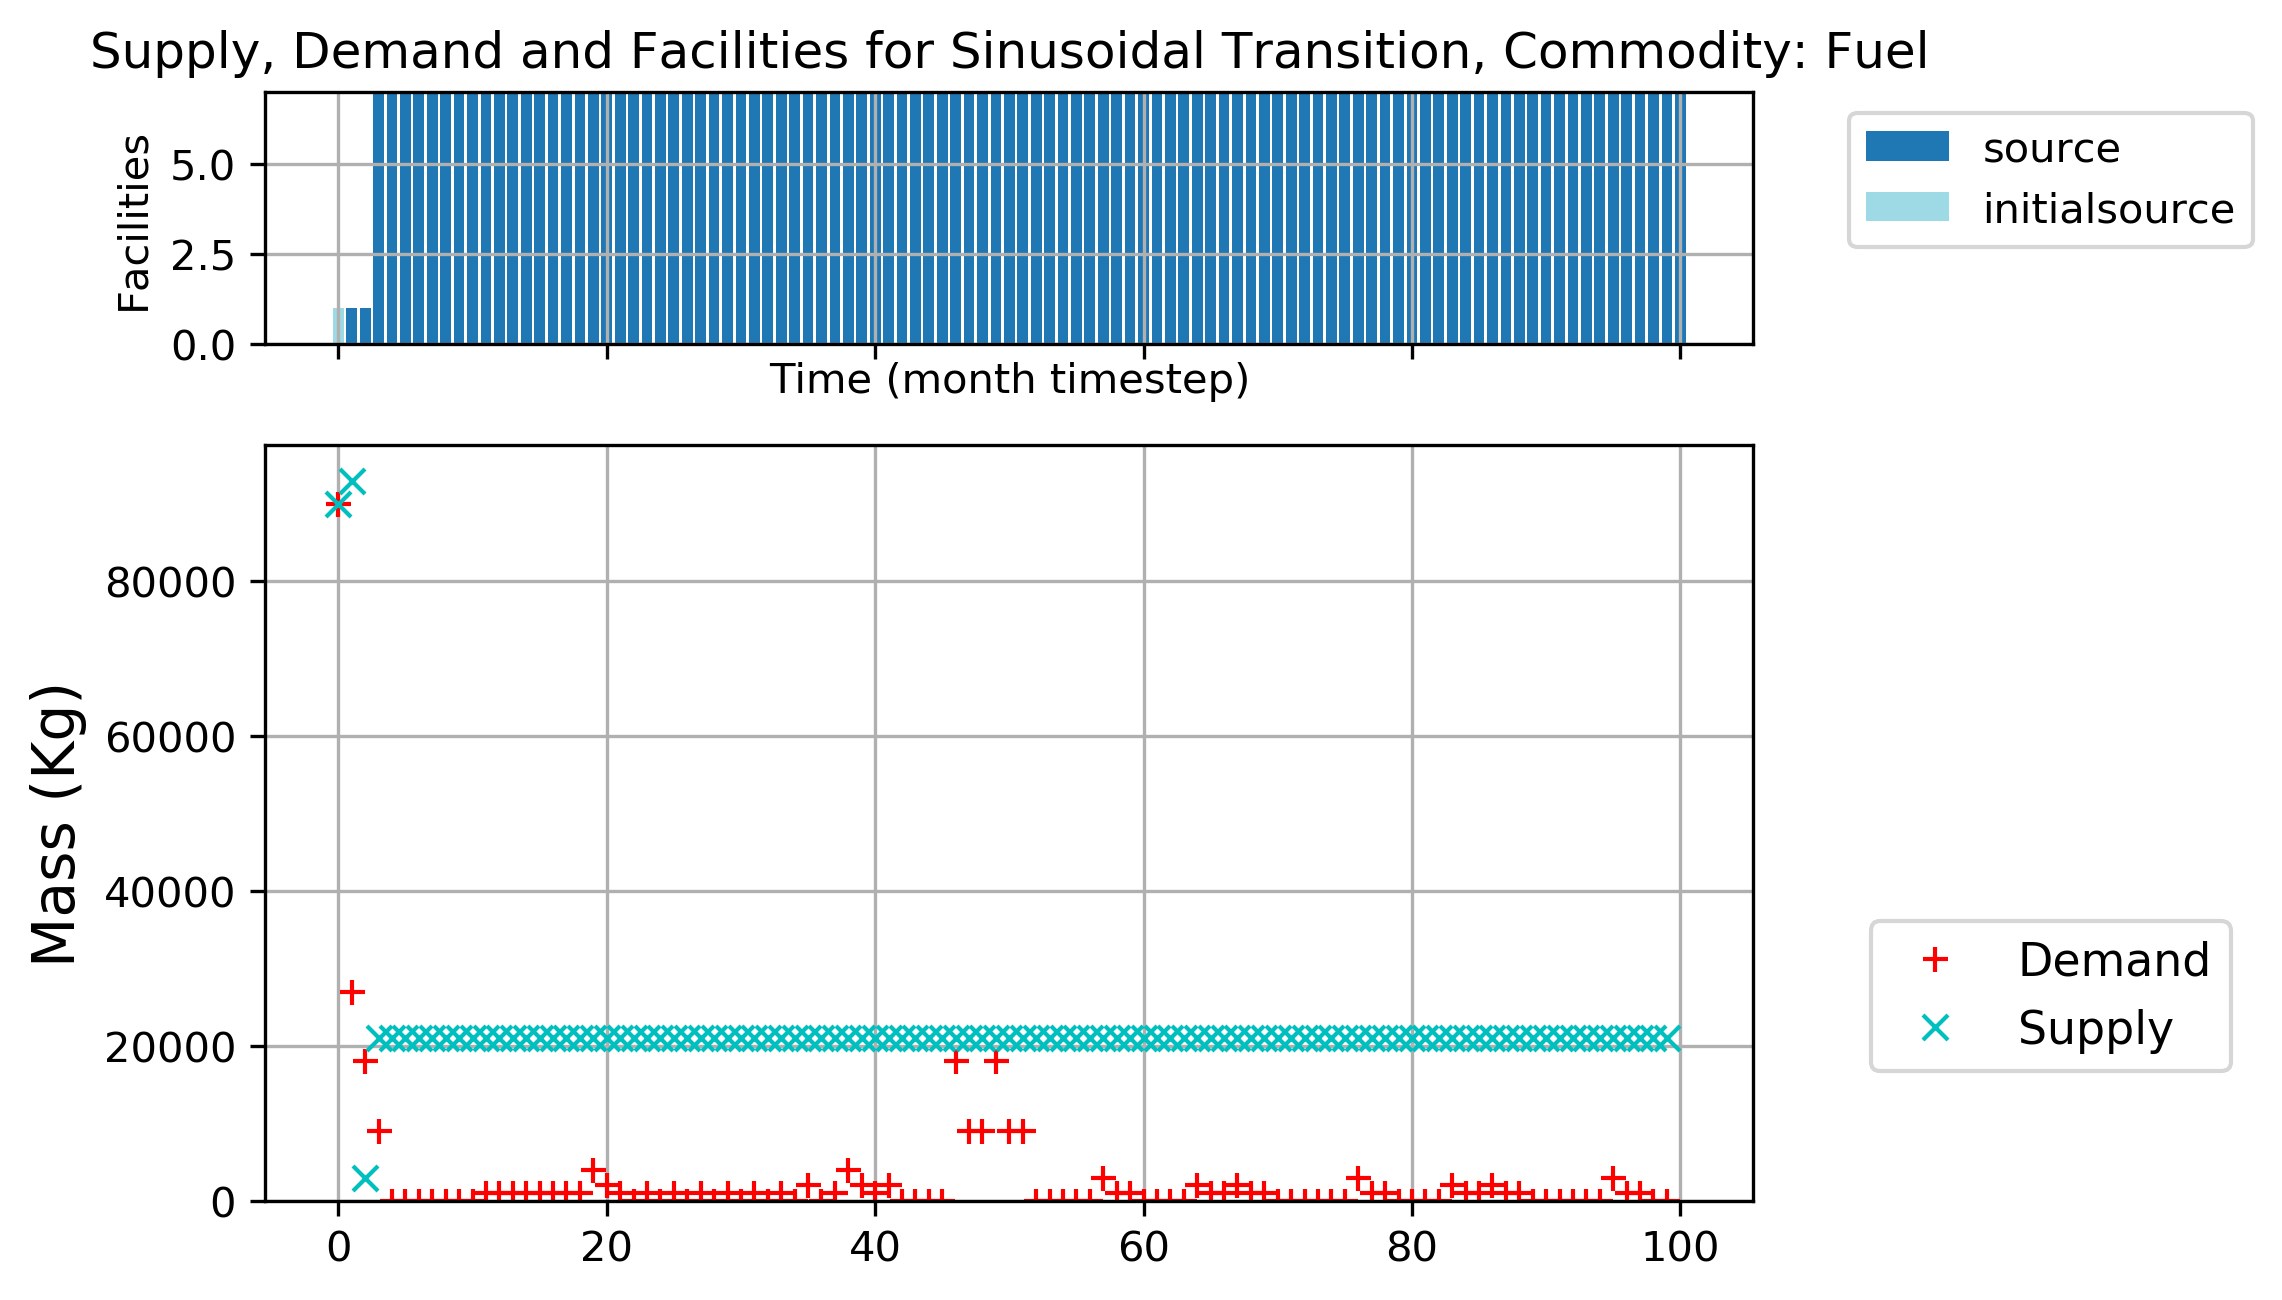
\includegraphics[width=\linewidth]{figures/sinetransition-fuel.png} 
        \caption{Fuel is demanded by reactors and supplied by source facilities.}
	    \label{fig:sinetransition-fuel}
    \end{subfigure}
    \begin{subfigure}[t]{0.65\textwidth}
        \centering
        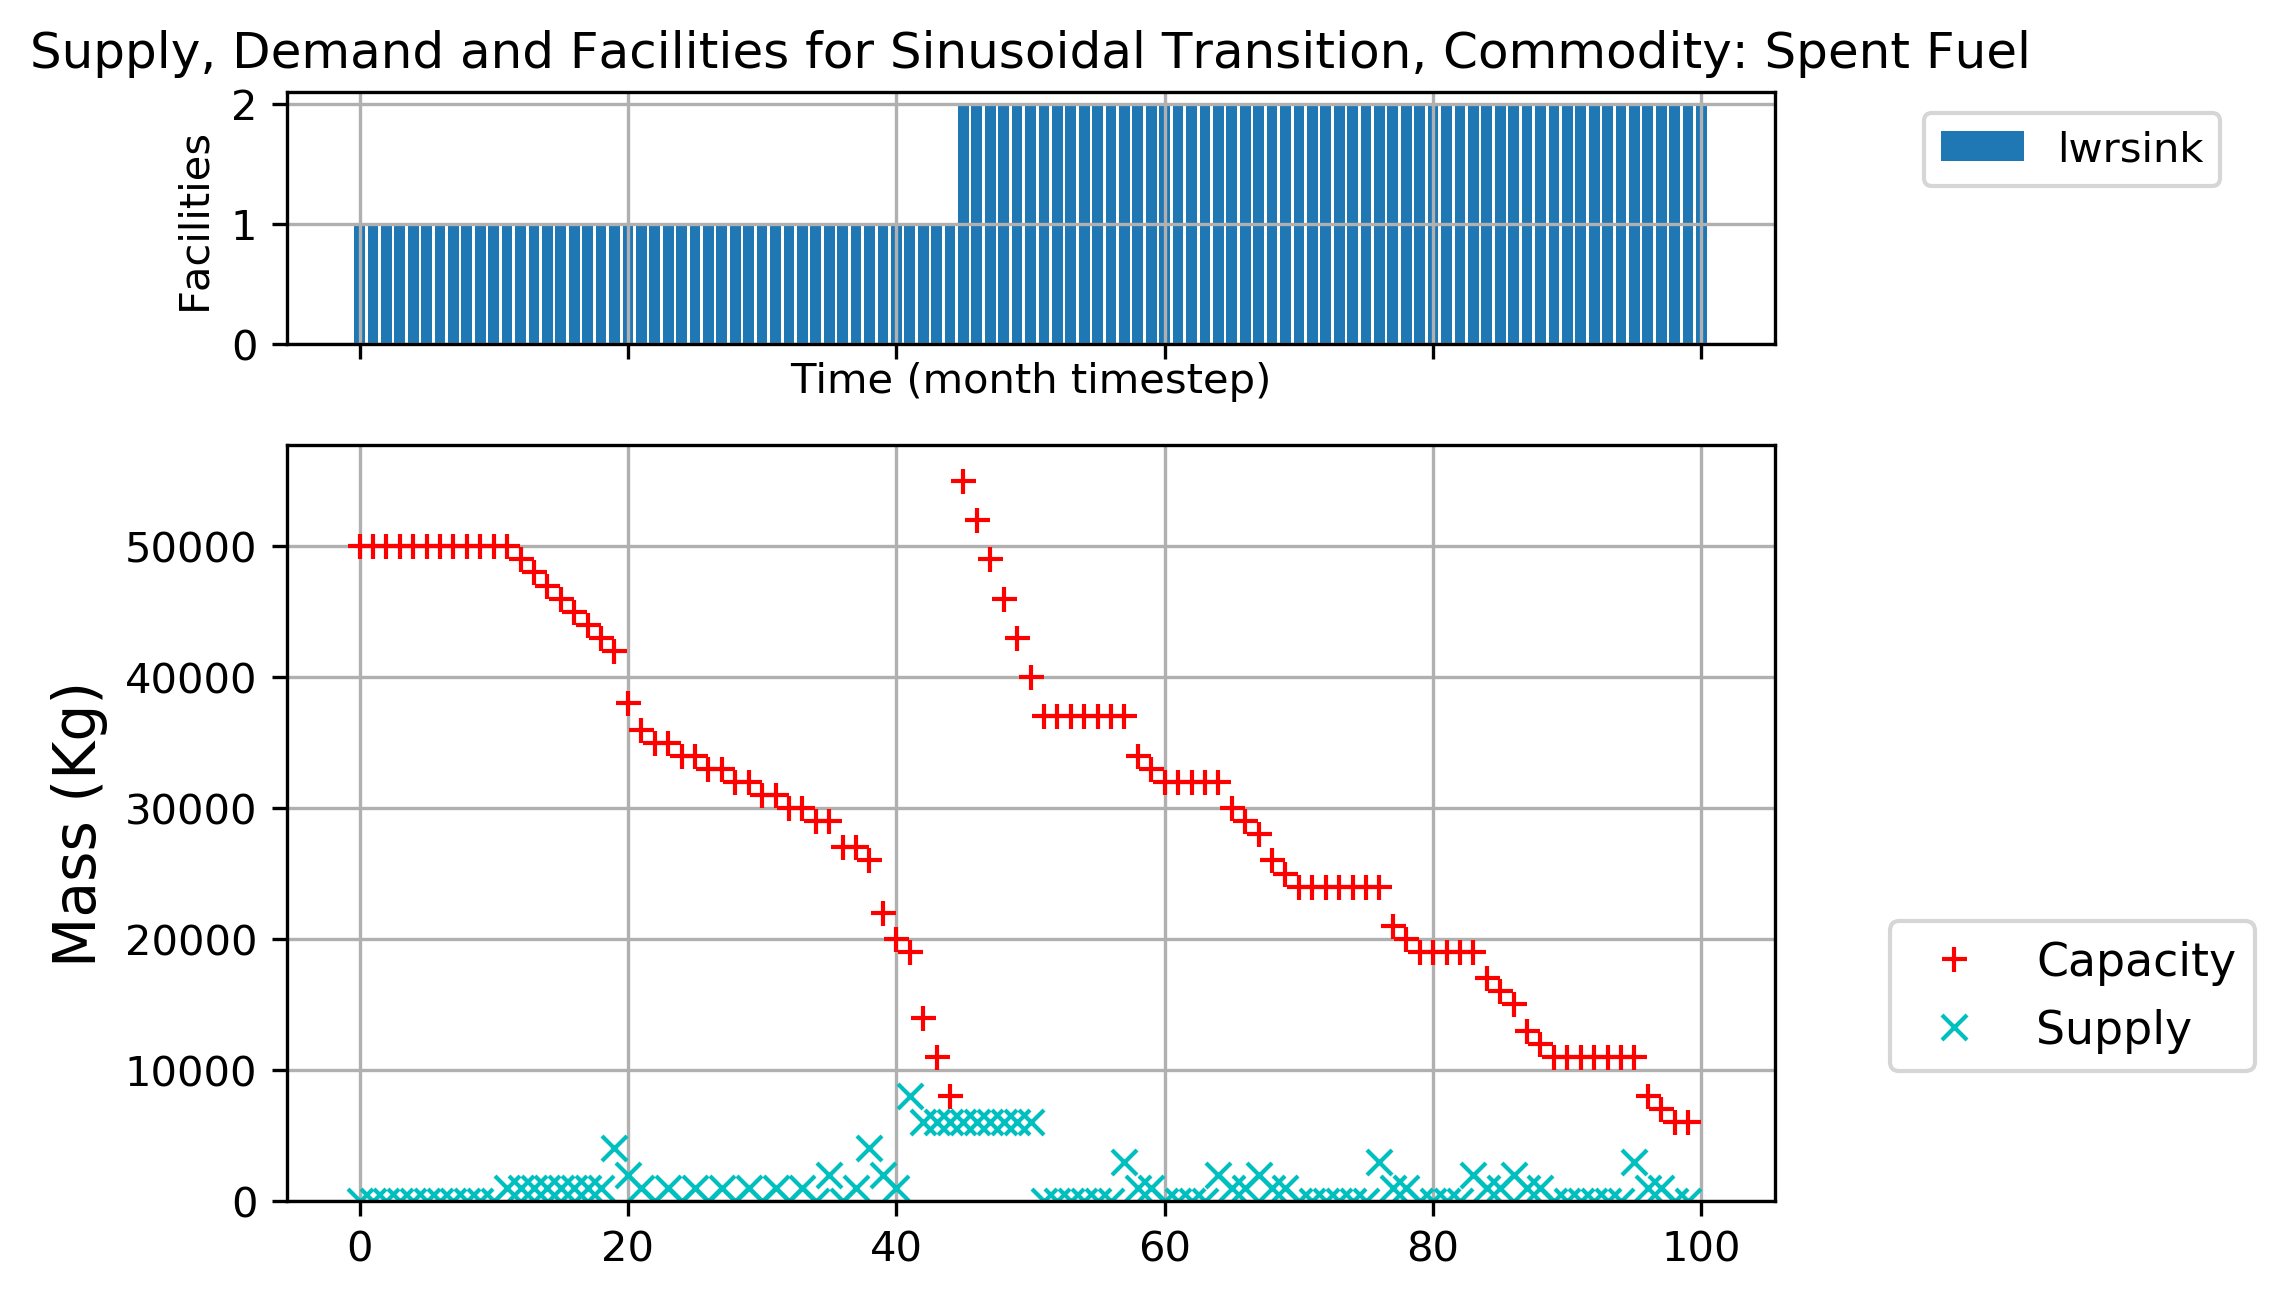
\includegraphics[width=\linewidth]{figures/sinetransition-spentfuel.png} 
        \caption{Spent Fuel is supplied by reactors and the capacity is provided by sink facilities.}
        \label{fig:sinetransition-spentfuel}
    \end{subfigure}
    \caption{Transition Scenario: Sinusoidal Power Demand}
\end{figure*}


In this section, a transition scenario with a linearly 
increasing power demand is shown. 
Table \ref{tab:transition-scenario-growing-power} shows the 
simulation parameters used in this transition scenario. 

Figures \ref{fig:growingtransition-power}, \ref{fig:growingtransition-fuel}
and \ref{fig:growingtransition-spentfuel} demonstrate the capability 
of \deploy to deploy reactor and supporting facilities to meet the
power demand and subsequently demanded secondary commodities 
for a linearly increasing power demand. 
The fast fourier transform method for predicting power demand is used for 
this scenario
which is identical to what was used for the constant power demand 
transition scenario. 
A smaller supply buffer could be used while still minimizing under supply. 

\subsection{\textbf{Transition Scenario: Sinusoidal Demand}}
In this section, a transition scenario with sinusoidal
power demand is shown. 
A sinusoidal power demand is the reflection of power demand in 
the real world where power usage is higher in the winter and summer
and lower in the spring and fall. 
Table \ref{tab:transition-scenario-sine-power} shows the 
simulation parameters used in this transition scenario. 

Figures \ref{fig:sinetransition-power}, \ref{fig:sinetransition-fuel}
and \ref{fig:sinetransition-spentfuel} demonstrate the capability 
of \deploy to deploy reactor and supporting facilities to meet the
power demand and subsequently demanded secondary commodities 
for a sinusoidal power demand. 

For a sinusoidal power demand, the use of the triple exponential method
for predicting demand is more effective than the 
fast fourier transform method which was used for the constant 
and linearly increasing power demand transition scenarios. 
This is because the triple exponential smoothing method excels in
forecasting data points for repetitive seasonal series of data.  

%%%%%%%%%%%%%%%%%%%%%%%%%%%%%%%%%%%%%%%%%%%%%%%%%%%%%%%%%%%%%%%%%%%%
\section{Conclusion}
This paper describes the capabilities of \deploy, demonstrates 
the use of \deploy for an assortment of transition scenarios: 
constant power demand, linearly increasing power demand and
sinusoidal power demand.  
It also provides insights on input parameter to ease the
setting up of larger transition scenarios that include many facilities. 
Future work includes setting up similar power demand transition 
scenarios for extended nuclear fuel cycles that incorporate reprocessing 
facilities etc. 
A more realistic transition scenario could be explored such as an 
increasing power demand that has a sinusoidal pattern to represent 
seasons in a year for a growing power demand trend. 

\nopagebreak
%%%%%%%%%%%%%%%%%%%%%%%%%%%%%%%%%%%%%%%%%%%%%%%%%%%%%%%%%%%%%%%%%%%%
\section{Acknowledgements}
This research is funded by the \gls{DOE} Office of 
Nuclear Energy's Nuclear Energy University Program 
(Project 16-10512, DE-NE0008567) 
"Demand-Driven Cycamore Archetypes". The authors want to thank 
members of the \gls{ARFC} group at the University of Illinois at 
Urbana-Champaign. 
We also thank our colleagues from the \Cyclus community, 
particularly those in the University of Wisconsin 
\gls{CNERG} and the University of South Carolina Energy Research 
Group (ERGS) for collaborative \Cyclus development.
%----------------------------------------------------------------%

%%%%%%%%%%%%%%%%%%%%%%%%%%%%%%%%%%%%%%%%%%%%%%%%%%%%%%%%%%%%%%%%%%%%
\bibliographystyle{ans}
\bibliography{bibliography}
\end{document}

